% By zmienic jezyk na angielski/polski, dodaj opcje do klasy english lub polish
\documentclass[polish,12pt]{aghthesis}
\usepackage[utf8]{inputenc}
\usepackage[usenames, dvipsnames]{color}
\usepackage{hyperref}
\usepackage{titlesec}
\usepackage{wrapfig}
\usepackage{lipsum}
\usepackage{float}
\usepackage{caption}

\setcounter{secnumdepth}{4}

\author{Wojciech Karpiel\\ Michał Hamuda\\ Filip Galas}

\titlePL{System rejestracji pacjentów - PRZEMEK\footnote{PRZEMEK - Produkt Rejestrujący Zapotrzebowanie na Ekspertyzę Medyczną Eliminując Kolejki}}
\titleEN{Patient registration system}

\fieldofstudy{Informatyka}

\supervisor{dr inż. Bartłomiej Śnieżyński}

\date{2017}

% Szablon przystosowany jest do druku dwustronnego, 
\begin{document}

\maketitle

\tableofcontents

\section{Cel prac i wizja produktu}
%\section{Project goals and vision}
\label{sec:cel-wizja}
\emph{Charakterystyka problemu, motywacja projektu (w tym przegląd
  istniejących rozwiązań prowadząca do uzasadnienia celu prac),
  wizja produktu, studium wykonalności i analiza zagrożeń.}
  
\subsection{Opis problemu}
Jednym z głównych zadań gabinetu lekarskiego jest przyjmowanie pacjentów na wizyty u lekarza. Zanim pacjent będzie mógł odbyć wizytę, zazwyczaj konieczna jest jego rejestracja. W ogólnym przypadku może ona przebiegać według poniższych kroków:

\begin{enumerate}
  \item Pacjent znajduje numer telefonu do recepcji gabinetu.
  \item Pacjent dzwoni do recepcji gabinetu.
  \item Recepcjonistka odbiera telefon.
  \item Pacjent przedstawia cel wizyty bądź nazwisko lekarza.
  \item Recepcjonistka odszukuje w grafiku możliwe terminy wizyty.
  \item Recepcjonistka podaje pacjentowi możliwe terminy wizyty.
  \item Pacjent wybiera termin wizyty.
  \item Recepcjonistka wpisuje termin do grafiku lekarza.
  \item Pacjent wpisuje termin do swojego kalendarza.
\end{enumerate}

W powyższym modelu wyróżniamy następujące niedogodności i problemy:
\begin{itemize}
%todo tu można jeszcze więcej głupot napisać
  \item Potrzeba znalezienia przez pacjenta numeru telefonu do gabinetu.
  \item Konieczność stałej obsługi linii telefonicznej przez recepcjonistkę w godzinach, w których pacjent ma możliwość rejestracji.
  \item Konieczność prowadzenia przez gabinet rejestru wizyt.
  \item Możliwość błędnego zapisania terminu lub zapomnienia przez pacjenta o umówionym terminie wizyty.
  \item Konieczność powiadomienia lekarza o nowej rezerwacji terminu wizyty w sposób ustny bądź pisemny.
  \item Brak natychmiastowego dostępu przez lekarza do danych pacjenta.
\end{itemize}

\subsection{Cel}
Stworzyć system eliminujący podane wyżej problemy i niedogodności, a w szczególności:

\begin{itemize}
  \item Dostarczyć pacjentowi możliwość samodzielnej rejestracji na wizytę u lekarza.
  \item Dostarczyć pacjentowi widok kalendarza pozwalający na ogląd dostępnych terminów i ich wybór oraz ogląd terminów zarezerwowanych wizyt.
  \item Dostarczyć lekarzowi widok kalendarza pozwalający ustalić godziny przyjęć, oznaczyć określone terminy jako niedostępne, zobaczyć zajęte przez pacjentów terminy oraz odwołać wizyty.
  \item Ułatwić lekarzowi dostęp do danych medycznych pacjenta zapisanego na wizytę.
  \item Dostarczyć recepcjonistce widok kalendarza pozwalający na sprawne poinformowanie rejestrującego się pacjenta o dostępnych terminach oraz zapisać go na wizytę.
  \item Umożliwić wpisywanie danych osobowych oraz wypełnianie formularzy medycznych przez rejestrującego się pacjenta bądź przez recepcjonistkę pozyskującą dane od pacjenta.
  \item Przypominać pacjentowi o umówionych terminach wizyty przez wysłanie SMS-a.
  \item Umożliwić automatyczne gromadzenie danych związanych z wizytami.
\end{itemize}

\subsection{Motywacja}
Motywacją była dla nas chęć zdobycia wiedzy z zakresu wytwarzania oprogramowania dla potrzeb medycznych, poznania specyfiki tej dziedziny, a także nauczenia się efektywnego wykorzystywania technologii używanych przez nas w procesie tworzenia produktu końcowego. Ponadto, jest to praca dyplomowa, na podstawie której dążymy do uzyskania tytułu inżyniera.

\subsection{Wizja produktu}
Rozwiązaniem wymienionych wyżej problemów będzie aplikacja, do której użytkownicy będą mieli dostęp poprzez przeglądarkę internetową.

Aplikacja będzie rozróżniała trzy typy użytkowników:
\begin{itemize}
    \item Administrator
    \item Lekarz
    \item Recepcjonistka
    \item Pacjent
\end{itemize}

Pacjent będzie mógł utworzyć swoje konto i zarejestrować się na wybrany termin wizyty spośród dostępnych terminów u wybranego lekarza. Recepcjonistka będzie mogła w imieniu pacjenta utworzyć jego konto i zarejestrować go na wizytę. Lekarz będzie mógł dodawać nowe terminy wizyt, przeglądać stan rezerwacji swoich wizyt i dane pacjentów. Administrator będzie posiadał wszystkie wymienione wyżej uprawnienia i będzie mógł pełnić rolę nadzorcy systemu.

Szczegółowe możliwości wykorzystania systemu przez każdy typ użytkowników są opisane w \emph{wymaganiach funkcjonalnych}.

Wszystkie dane dot. pacjentów, lekarzy, dostępnych terminów wizyt i rezerwacji będą gromadzone w bazie danych.

\subsection{Studium wykonalności}
Technologie wymienione w \hyperref[subsec:analizaTechnologiczna]{\emph{Analizie technologicznej}} zostały uzgodnione przed rozpoczęciem prac z Klientem i pozostałymi zespołami --- było to konieczne ze względu na wysokie sprzężenie modułów przygotowywanych przez zespoły. Dlatego jesteśmy przekonani że technologie zostały dobrane poprawnie i produkt jest wykonalny ze względu na dobrane technologie.

Ograniczenia czasowe na wykonanie produktu zostały rozważone (miało to wpływ między innymi na \hyperref[subsec:wykorzystane-technologie-baza]{schemat bazy danych}).

Ponadto, przeprowadziliśmy analizę zagrożeń, której wyniki przedstawiamy poniżej.

\subsubsection{Analiza zagrożeń}
Możemy wyróżnić następujące czynniki ryzyka:
\begin{itemize}
  \item Rozbieżności między zespołami, a w szczególności:
  \begin{itemize}
    \item niespójna wizja produktu,
    \item niespójne API,
    \item porzucenie swojej części produktu lub niezrealizowanie wspólnych funkcjonalności przez którąkolwiek z zależnych grup.
  \end{itemize}
  Wszystkie wyżej wymienione zdarzenia uniemożliwiłyby powstanie w pełni działającego produktu, ze względu na to że poszczególne moduły są od siebie współzależne. Ryzyko wystąpienia rozbieżności można zminimalizować poprzez częste uzgadnianie między zespołami wizji produktu oraz API tych funkcjonalności, które udostępniane są zależnym modułom. Takie dyskusje powinny odbywać się nie tylko przed rozpoczęciem prac implementacyjnych, ale także w ich trakcie.
  \item Nieefektywne wykorzystanie technologii:
  \begin{itemize}
    \item front-endowych (\href{https://getbootstrap.com/}{Twitter Bootstrap}),
    \item komunikacyjnych (HTTP Api),
    \item zapewniających bezpieczeństwo (\href{https://jwt.io/}{JWT}).
  \end{itemize}
  Wyżej wymienione zdarzenia skutkowały by powstaniem brzydkiego, ciężkiego w obsłudze lecz działającego produktu.
\end{itemize}
\section{Zakres funkcjonalności}
%\section{Functional scope}
\label{sec:zakres-funkcjonalnosci}

\emph{Kontekst użytkowania produktu (aktorzy, współpracujące systemy)
  oraz specyfikacja wymagań funkcjonalnych i niefunkcjonalnych.}
  
\subsection{Aktorzy}
W aplikacji będziemy rozróżniać trzy typy użytkowników:
\begin{itemize}
    \item Administrator
    \item Lekarz
    \item Recepcjonistka
    \item Pacjent
\end{itemize}
Ich możliwości wykorzystania systemu są opisane w \emph{wymaganiach funkcjonalnych}. 

\subsection{Przypdaki użycia}
    \begin{figure}[H]
        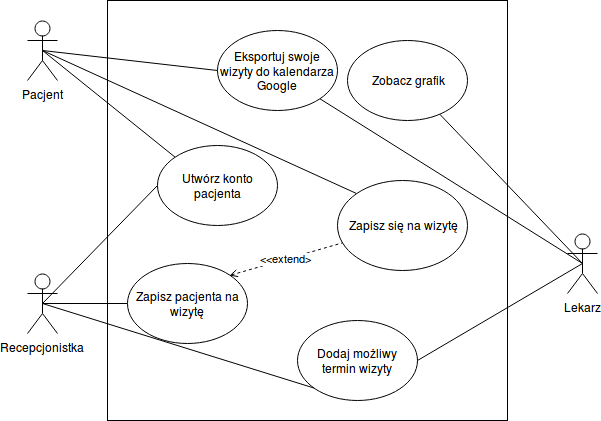
\includegraphics[width=\textwidth]{use-case-v1}
        \caption{Przypdaki użycia systemu rejestracji pacjentów}
    \end{figure}
    
\subsection{Współpracujące systemy}
\emph{Przemek} współpracuje z \emph{Modułem komunikacji ze sprzętem medycznym} oraz \emph{Systemem wspomagającym prowadzenie gabinetu lekarskiego} tworząc rozbudowany system medyczny.

%opisy przeklejone z dyplom.iisg.agh.edu.pl
%coś więcej sie dowiemu pewno dopiero na sporkaniu 10.04 lub 11.04
\subsubsection{Moduł komunikacji ze sprzętem medycznym}
Moduł komunikacji ze sprzętem medycznym takim jak aparat USG na przykład firm GE, Samsung, Toshiba lub Philips. Moduł umożliwia pobieranie wyników badań w tym zdjęć w formacie DICOM z urządzeń medycznych do systemu wspomagającego prowadzenie gabinetu lekarskiego.
\subsubsection{System wspomagający prowadzenie gabinetu lekarskiego}
System wspomagający prowadzenie gabinetu lekarskiego zapewnia następujące funkcjonalności
\begin{itemize}
  \item Obsługa wizyty pacjenta (wywiad, zalecenia itp.)
  \item Badania lekarskie (skierowanie, odbiór wyników - obrazki i opis)
\end{itemize}

\subsection{Specyfikacja wymagań}

\subsubsection{Wymagania funkcjonalne}
\small\emph{Przedstawione wymagania są opracowane na podstawie wymagań gabinetu z USG, przez co wymagania specyficzne dla tego rodzaju gabinetu mieszają się z  wymaganiami dla gabinetów lekarskich w ogólności}
%rzeczy dodane do podstawi z e-maila kończą się tagiem %[DW]
\begin{itemize}
    \item System rejestracyjny będzie oparty na bazie danych pacjentek \begin{enumerate}
      \item Imię
      \item Nazwisko
      \item Data urodzenia
      \item Ciąża (kolejny numer)
      \item Poród (kolejny numer)
      \item PESEL
      \item Adres
      \item Telefon
      \item Email
      \item Osoby upoważnione
      \item Lekarz kierujący
      \item Miejsce pracy
      \item Kategoria położnicza (norma; wada głowy/szyi; wada klatki piersiowej; wada serca; wada brzucha; wada kończyn; wada kręgosłupa; nieprawidłowość łożyska; małowodzie; wielowodzie; aneuploidia; inne-dodaj kategorię)
      \item Kategoria ginekologiczna (norma; zmiany w szyjce; zmiany w macicy; zmiany w jajnikach; zmiany w jajowodach; onko-ginekologia; inne-dodaj kategorię)
      \item \emph{Klasyfikacja kto jest lekarzem prowadzącym pacjentkę, czy pacjentka jest na usg, czy jest na wizytę, kto wykonywał badanie poprzednie}
    \end{enumerate}
    \item Recepcja rejestrując pacjentkę telefonicznie wprowadza: \begin{enumerate}
      \item Imię - wymagane
      \item Nazwisko - wymagane
      \item Nr telefonu - wymagane
      \item Nr pesel - opcjonalne
      \item Klasyfikuje pacjentkę: - opcjonalnie \begin{itemize}
          \item usg genetyczne \begin{itemize}
              \item pierwszy trymestr
              \item drugi trymestr
              \item trzeci trymestr
              \item przepływy maciczne
              \item ocena dobrostany – Biometria
              \item usg kontrolne – monitorowanie nieprawidłowości
              \item echo serca płodu –ciąża zdrowa
              \item usg drugiej opinii
              \item usg nieprawidłowości
          \end{itemize}
          \item usg ginekologiczne
          \item procedura diagnostyczna (biopsja kosmówki, amniopukcja)
          \item wizyta lekarska (pacjentka ginekologiczna)
          \item wizyta lekarska rozszerzona \begin{itemize}
              \item założenie wkładki IUD
              \item zabieg laserowy
              \item zabieg
          \end{itemize}
          \item wizyta lekarska w ciąży
          \item wizyta lekarska w wysokiej ciąży (wizyta + ktg)
      \end{itemize}
      \item Uwagi - opcjonalnie
      \item adres e-mail - opcjonalnie 
    \end{enumerate}
    Do zarejestrowania pacjentki należy wpisać \textbf{wymagane dane} – bez tych danych miejsce nie może być zarejestrowane.
    \item Z listy pacjentek w bazie danych filtrowanie pacjentek po:  (z poziomu recepcji) \begin{itemize}
        \item Nazwisku
        \item Dacie urodzenia
        \item Peselu
        \item Numerze telefonu
    \end{itemize}
    \item Kalendarz rejestracyjny \begin{itemize}
        \item dostosowany do danego lekarza
    \end{itemize}
    \item Z poziomu administratora \begin{itemize}
        \item ustala i formułuje grafik na dany okres czasu wg dyspozycyjności lekarza
        \item wprowadza daty i godziny przyjęć poszczególnych lekarzy 
        \item ma możliwość wprowadzać przerwy w przyjęciach 
        \item klasyfikowanie lekarzy do grup (w zależności od wykonywanej procedury)
    \end{itemize}
    \emph{Takie rozwiązanie skróci czas rejestracji do minimum – pacjentka podaje temat wizyty (procedury) i w proponowanych lekarzach pojawiają się odpowiednie nazwiska}
    \item Z poziomu lekarza \begin{itemize}
        \item widok kalendarza przyjęć
        \item możliwość zarejestrowania pacjentki 
        \item identyfikacja kto rejestruje pacjentkę
        \item formułuje swój grafik i ustala możliwe godziny przyjęć %[DW]
    \end{itemize}
    \item Z poziomu pacjenta \begin{itemize} %[DW] - cała sekcja
      \item samodzielnie tworzy konto
      \item samodzielnie rejestruje się na wizytę u lekarza
      \item samodzielnie podaje swoje dane osobowo-medyczne (tych samych które wprowadza recepcja rejestrując pacjenta)
      \item widok kalendarza swoich umówionych wizyt
      \item widok kalendarza dostępnych terminów wizyty podczas rejestracji
      \item ustawia przypomnienie dla siebie o zarezerwowanych terminach wizyt
    \end{itemize}
    \item Z poziomu recepcji \begin{itemize}
        \item każda osoba rejestrująca zalogowana na własne konto lub posiadająca własny login
        \item recepcja ma możliwość rejestrowania pacjentów z różnych komputerów
        \item stworzenie blokowania danego terminu w momencie najechania na termin (aby uniknąć dublowania rejestracji równocześnie przez dwie panie w recepcji)
        \item Możliwa rejestracja z poziomu kalendarza  - najechanie na dany dzień i daną godzinę – kliknięcie zarejestruj termin – przeniesienie do formularza wprowadzanie pacjentki
        \item Weryfikowanie dublowanych terminów  ( w zależności od klasyfikacji pacjentki)  \\
        \emph{Pacjentki które prowadzą ciąże mają zarezerwowane w kalendarzu kilka terminów wizyt. Pacjentki na usg prenatalne wpisują się kilkukrotnie do wielu lekarzy – takie pacjentki porzebujemy zweryfikować.} \\
        Pacjentki zakwalifikowane np.: usg genetyczne pierwszy trymestr (jeśli jest kilka takich o takiej samej dacie urodzenia to wyskakuje na czerwono w momencie rejestracji)
        \item stworzenie wspólnych powiązań pomiędzy lekarzami ultrasonografistami (grup lekarzy pracujących wspólnie) aby można było znaleźć wolne miejsce na daną procedurę \\
        \emph{Pacjentka dzwoni i chce się zarejestrować na usg prenatalne I trymestru i powinny wyskoczyć wolne terminy np. Od dziś do ustalonej daty, we wszystkich grupach docelowych, czyli u wszystkich lekarzy wykonujących usg prenatalne}
        \item każdy lekarz osobny kalendarz  tzn. odstępy między godzinami są różne u lekarzy o różne w każdej godzinie. \\
        8:00 8:20 8:40 9:00  9:30 10:00 10:20
        \item ważne jest aby formularz był stały ponieważ każdy ma inny system przyjmowania i wpisywanie samemu godzin pracy wprowadza duże zamieszanie, ilość pacjentek na dany dzień przyjęciowy się nie zgadza. 
    \end{itemize}
    \item SMS-y potwierdzające \\
    Wysyłanie smsów potwierdzających zarezerwowany termin po zarezerwowaniu terminu oraz potwierdzających wizytę na kilka dni wcześniej (ilość dni możliwa do regulacji) 
\end{itemize} 
%koniec listy wymgaań funkcjonalnych
 
\subsubsection{Wymagania niefunkcjonalne}
\begin{itemize}
    \item Aplikacja ma wykorzystywać \href{https://getbootstrap.com/}{Twitter Bootstrap} do stworzenia interfejsu użytkownika --- jest to ustalone ze względu na wymaganie zachowania spójności wyglądu z produktami zależnymi.
    \item W warstwie bazodanowej ma być używana relacyjna baza danych --- jest to ustalone ze względu na kompatybilność z produktami zależnymi.
    \item Aplikacja ma działać w przeglądarce internetowej.
    \item Aplikacja ma działać na komputerach stacjonarnych, laptopach oraz tabletach.
    \item Aplikacja ma działać dla wielu współbieżnych użytkowników.
    \item Aplikacja ma być łatwa w obsłudze dla personelu gabinetu lekarskiego oraz pacjentów.
\end{itemize}


\section{Wybrane aspekty realizacji}
%\section{Selected realization aspects}
\label{sec:wybrane-aspekty-realizacji}

\emph{Przyjęte założenia, struktura i zasada działania systemu,
  wykorzystane rozwiązania technologiczne wraz z uzasadnieniem
  ich wyboru, istotne mechanizmy i zastosowane algorytmy}

\subsection{Analiza technologiczna}
\label{subsec:analizaTechnologiczna}
Analiza odbywa się według warstw logicznych aplikacji opisanych w \emph{Wizji rozwiązania}

\subsubsection{Aplikacja użytkownika}
Aplikacja będzie działała w przeglądarce internetowej. \\
Wykorzystane technologie:
\begin{itemize}
  \item \href{https://pl.wikipedia.org/wiki/HTML}{HTML}
  \item \href{https://pl.wikipedia.org/wiki/JavaScript}{JavaScript}
  \item \href{https://jwt.io/}{JWT} - dla bezpieczeństwa komunikacji i utrzymania sesji użytkownika
\end{itemize}

Dla polepszenia satysfakcji klienta i uspójnienia wyglądu z innmi modułami wykorzystamy zręby
\begin{itemize}
  \item \href{https://getbootstrap.com/}{Twitter Bootstrap}
\end{itemize}

\subsubsection{Serwer do komunikacji z innymi modułami}
Będzie to serwer HTTP API, komunikaty będziemy przesyłać w standardzie JSON \\
Wykorzystane technologie:
\begin{itemize}
  \item \href{https://pl.wikipedia.org/wiki/Hypertext_Transfer_Protocol}{HTTP} - zwłaszcza metody \emph{GET} i \emph{POST}
  \item \href{http://www.json.org/}{JSON}
  \item \href{https://www.oracle.com/java/index.html}{Java}
\end{itemize}

\subsubsection{Baza danych}
\label{subsec:wykorzystane-technologie-baza}
Wykorzystamy relacyjną bazę danych - dane pacjentów i rejestracji są relacyjne. Problemem tego pojeścia jest mała elastyczność. \\
Elastyczność jest wymagana ze względu na potrzebę wspierania różnych formularzy dla pacjentów w zależności od typu gabinetu lekarskiego oraz różnych formularzy dla pacjentów w zależności od potrzeb lekarza. \\
Ten problem rozwiążemy przechowująć pliki \emph{JSON}-owe w bazie danych. Jest to rozwiązanie kiepsce lecz usprawiedliwione prostotą implementacji. Stworzenie i poprawna implementacja relacyjnego modelu danych posiadającego wymaganą elastyczność wymagało by więcej czasu niż jesteśmy w stanie poświęcić pracy inżynierskiej \\
Wykorzystane technologie:
\begin{itemize}
  \item \href{https://www.postgresql.org/}{PostreSQL}
\end{itemize}


\subsection{Dziedzina problemu}

\subsubsection{Przeglądarka internetowa}
Produktem jest przeglądarka internetowa. Przeglądarka to  program komputerowy służący do pobierania i wyświetlania stron internetowych udostępnianych przez serwery WWW\footnote{\href{https://pl.wikipedia.org/wiki/Przeglądarka_internetowa}}.

\begin{figure}[H]
    \centering
    \begin{minipage}{0.45\textwidth}
        \centering
        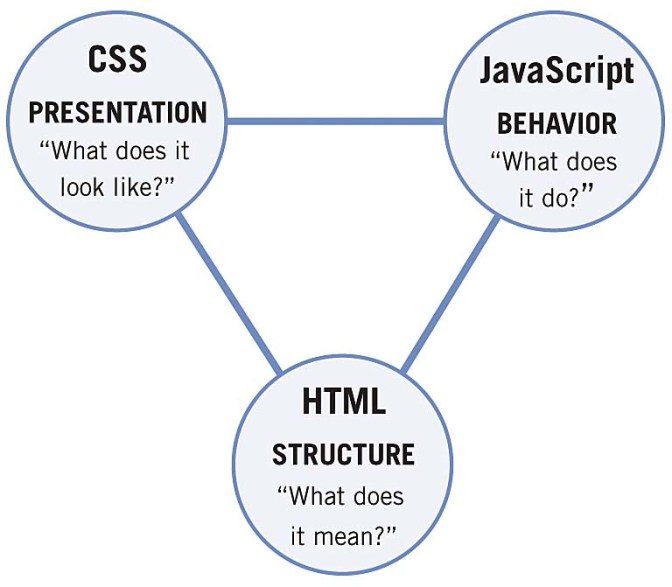
\includegraphics[width=0.9\textwidth]{html-css-js} % first figure itself
        \caption{Strony internetowe są tworzone z użyciem HTML-a, CSS-a i JavaScript-a}
    \end{minipage}\hfill
    \begin{minipage}{0.45\textwidth}
        \centering
        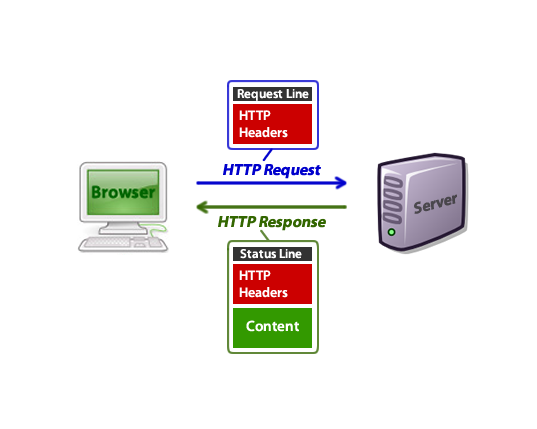
\includegraphics[width=0.9\textwidth]{http_diagram} % second figure itself
        \caption{Przeglądarka internetowa pobiera strony internetowe używając protokołu HTTP}
    \end{minipage}
\end{figure}


\subsection{Wstęp - zarys architektury systemu}
Na architekturę produktu składa się:
\begin{itemize}
    \item Aplikacja przeglądarkowa (front-end)
    \item Aplikacja strony serwerowej (back-end)
    \item Baza danych
\end{itemize}


\begin{figure}[H]
    \centering
    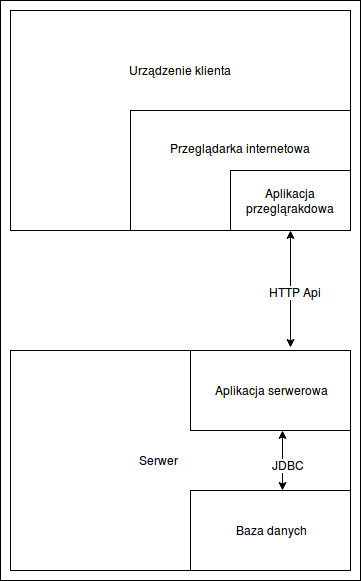
\includegraphics{komunikacja-serwer-klient-okolny}
    \caption{Front-end jest aplikacją wykonującą się na urządzeniu użytkownika. Zapytania o dane i wysyłanie danych do aplikacji strony serwerowej za pomocą HTTP Api. Strona serwerowa komunikuje się z bazą danych za pomocą JDBC}
    \label{fig:my_label}
\end{figure}




\subsubsection{Zarys architektury aplikacji serwerowej}
\begin{figure}[H]
    \centering 
    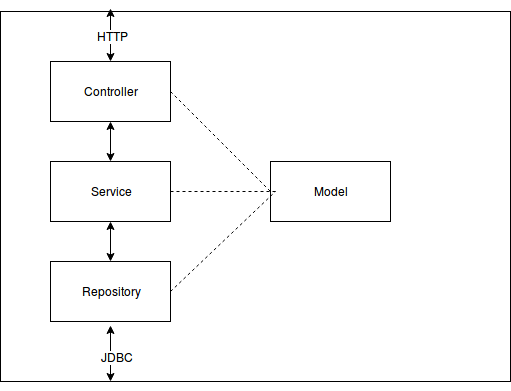
\includegraphics[width=\textwidth]{backedn-schema}
    \caption{Poglądowy schemat architektury aplikacji serwerowej}
\end{figure}
    
\begin{itemize}
    \item Controller - warstwa odpowiedzialna za odbieranie zapytań HTTP i przetwarzanie ich na obiekty JVM-owe oraz za przetwarzanie odpowiedzi (obiektów JVM-owych) na waidomości HTTP i odsyłanie ich.
    \item Service - warstwa pośrednicząca międzu Controller-em a Repository-em. Przetwarza zapytania otrzymane od Controllera na zapytania dla Repository i przetwarza odpowiedzi od Repository na odpowiedzi dla Controller-a.
    \item Repository - warstwa odpowiedzialna za wykonywanie zapytań do bazy danych.
    \item Model - wspóny dla wyżej wymienionych warstw sposób reprezentacji encji jako obiektów JVM-kowych, który może być przetworzony na JSON-a (na potrzeby HTTP API) lub repotezentację bazodanową (na potrzeby bazy danych). Umożliwia komunikację pomiędzy Controller-em, Servic-em i Repository-em.
\end{itemize}

\subsubsection{Zarys architektury aplikacji przeglądarkowej}
\begin{figure}[H]
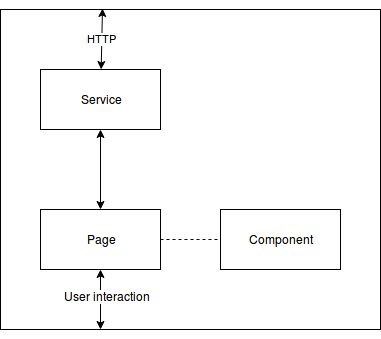
\includegraphics[width=\textwidth]{front-schema}
\caption{Poglądowy schemat architektury aplikacji przeglądarkowej}
\end{figure}
\begin{itemize}
    \item Service - serwisy odpowiadają za wysyłanie zapytań do aplikacji serwerowej i odbieranie odpowiedzi
    \item Page - Trasowalna strona wyświatlana użytkownikowi
    \item Component - Strony korzystają z komponentów
\end{itemize}



\subsection{Baza danych}
Wykorzystano bazę PostgresSQL. 
\begin{figure}[H]
\caption{Schemat bazy danych jest tworzony ad-hoc przy starcie aplikacji przez \emph{Hibernate}-a}
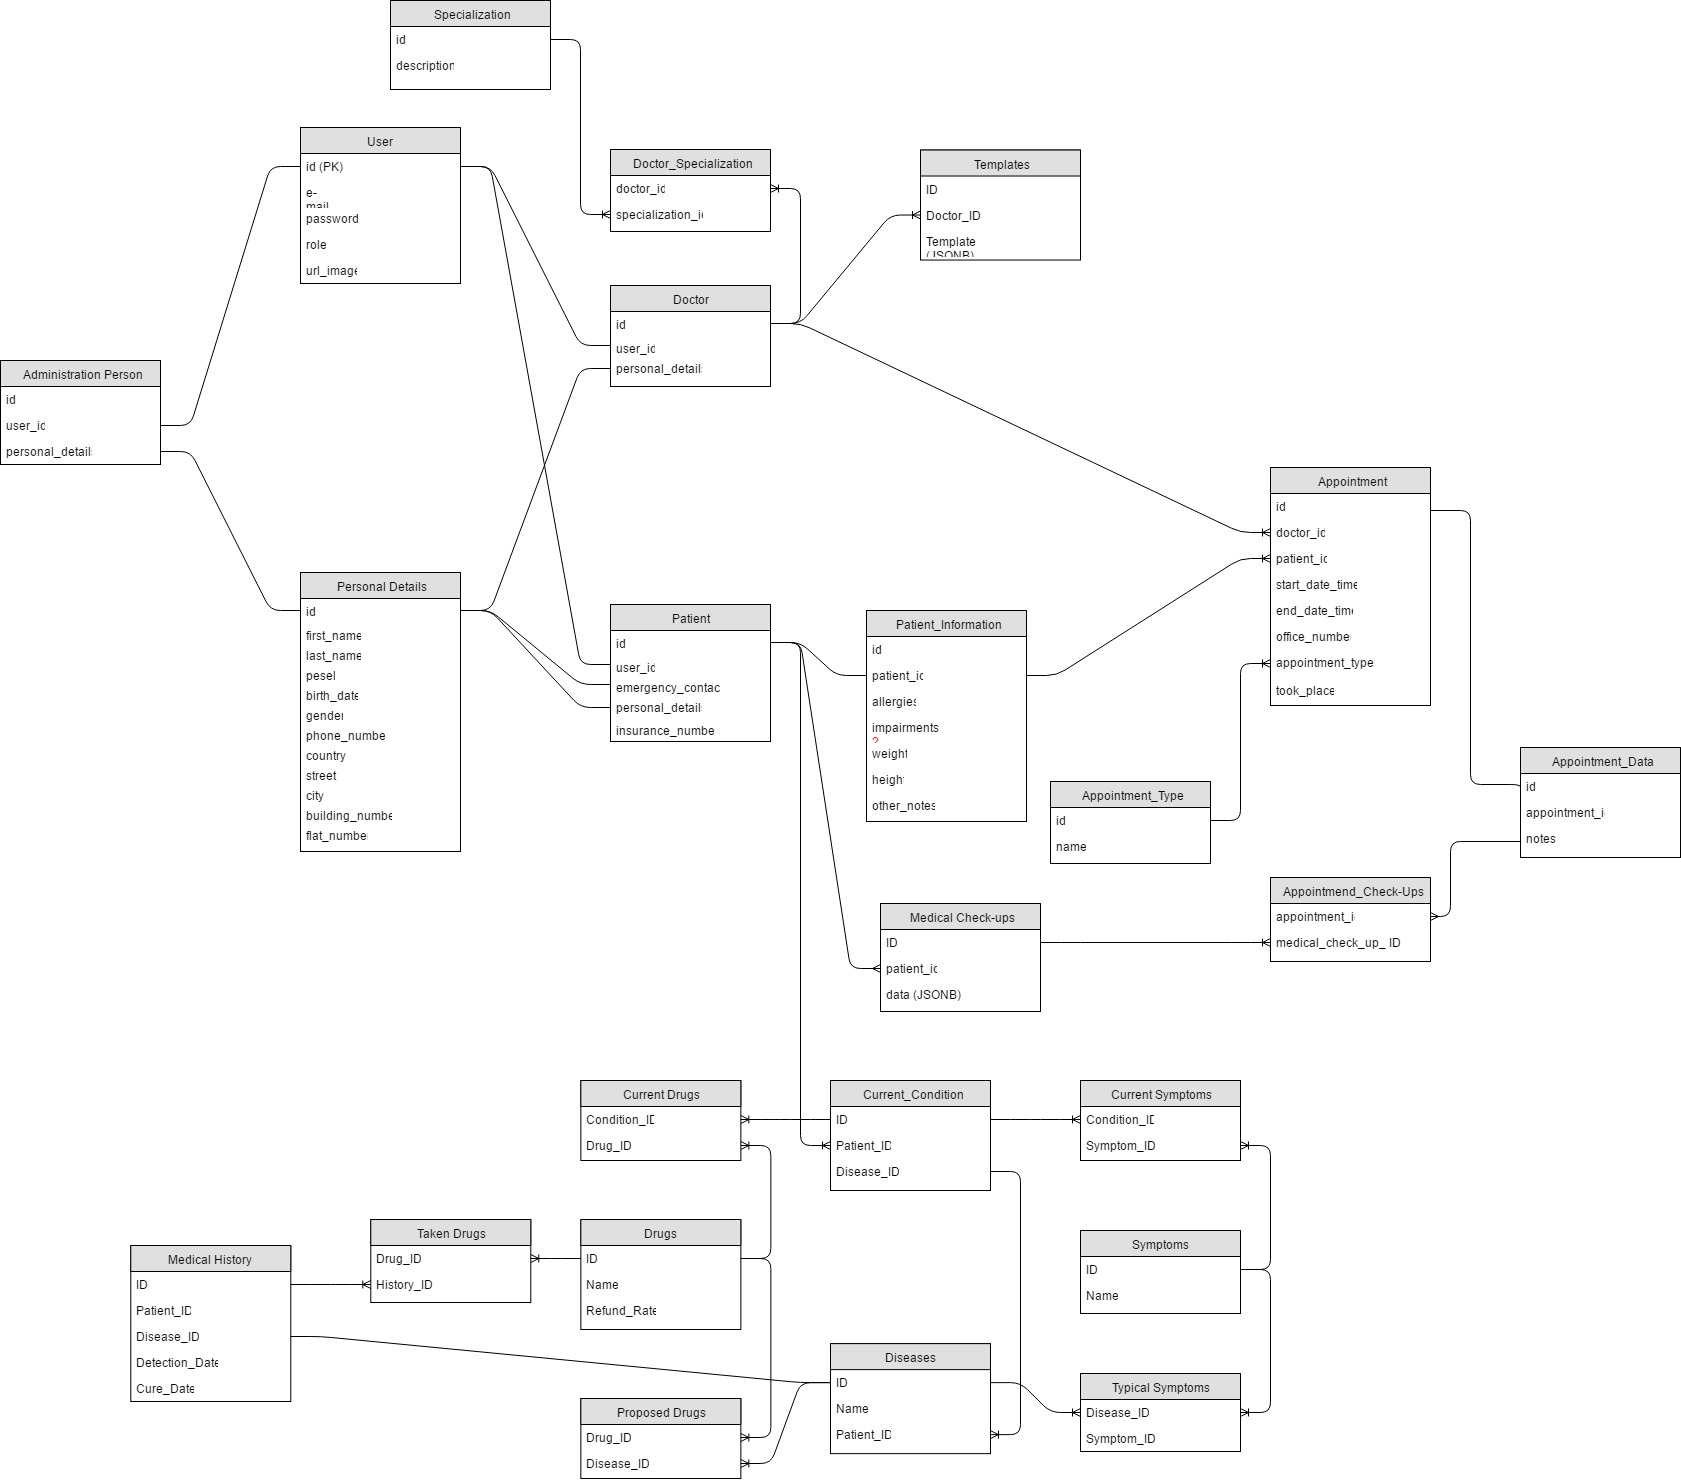
\includegraphics[width=\textwidth]{db-schema}
\end{figure}

\subsection{Aplikacja strony serwerowej}
\subsubsection{Technologie}
Wykorzystano język programowania Java, zrębów Spring i Hibernate.
\paragraph{Spring} pozwala na:
\begin{itemize}
    \item odbieranie i wysyłanie zapytań HTTP
    \item używanie CRUD-owego API do bazy danych
\end{itemize}
\paragraph{Hibernate} pozwala na:
\begin{itemize}
    \item Utworzenie schematu bazy danych na podstawie klas Java-owych
    \item serializację i zapis obiektów Java-owych
    \item odczyt z bazy obiektów Java-owuch
\end{itemize}
\subsubsection{Modelowane encje}
    \paragraph{Timeslot} - możliwy termin wizyty u danego lekarza.
    \begin{figure}[H]
    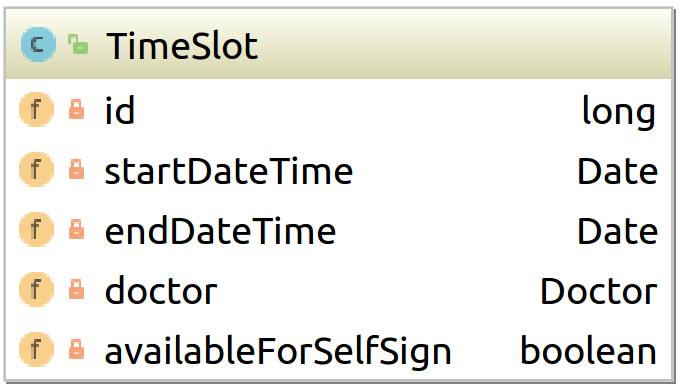
\includegraphics[width=0.7\textwidth]{TimeSlot}
    \caption{Nie zawiera informacji czy termin jest zarezerwowany, może być interpretowany jako czas w którym lekarz na pewno jest w pracy}
    \end{figure}
    \paragraph{Appointment} - Zarezerwowany termin u wizyty
    \begin{figure}[H]
    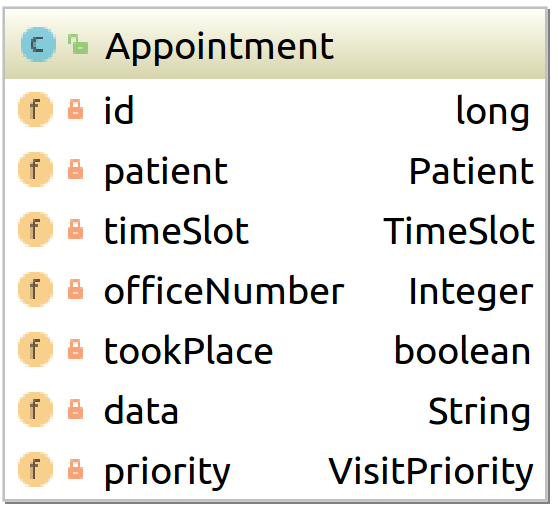
\includegraphics[width=0.7\textwidth]{Appointment}
    \caption{Zawiera szczegóły rezerwacji, jak na przykład dane pacjenta czy priorytet wizyty.
    Zawiera w sobie \emph{TimeSlot} - czyli informację o terminie i lekarzu przyjmującym wizytę}
    \end{figure}
    \paragraph{Doctor} - lekarz 
    \begin{figure}[H] 
    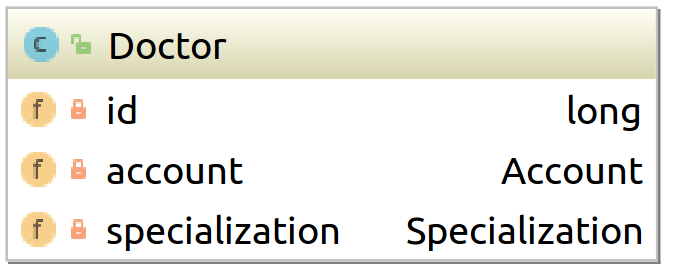
\includegraphics[width=0.7\textwidth]{Doctor} 
    \caption{Encja lekarza odpowiada jednej jego specjalizacji}
    \end{figure}
    \paragraph{Patient} - pacjent 
    \begin{figure}[H]
    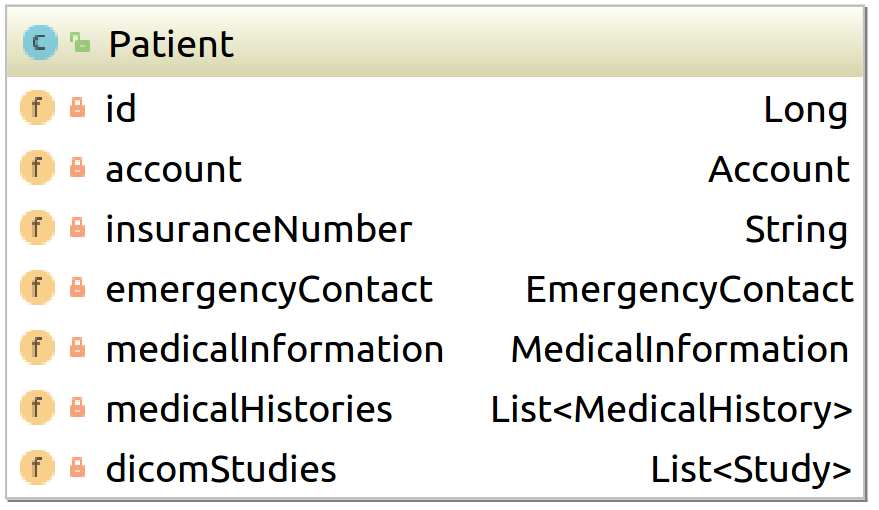
\includegraphics[width=0.7\textwidth]{Patient}
    \end{figure}
    \paragraph{Account} - konto w systemie 
    \begin{figure}[H]
    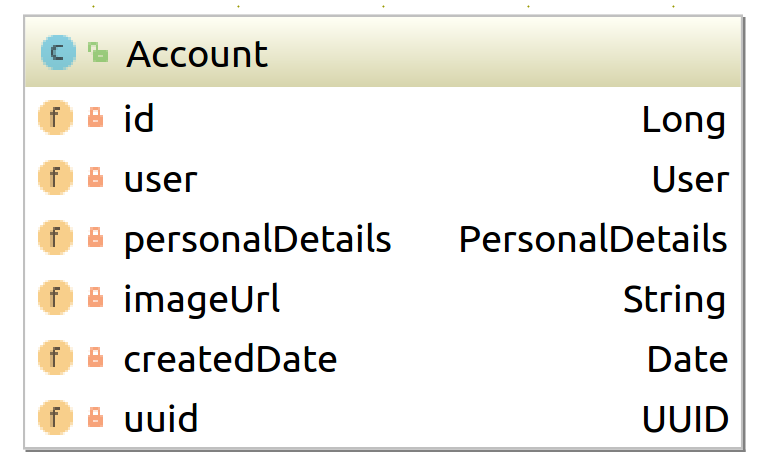
\includegraphics[width=0.7\textwidth]{Account}
    \caption{Konto nie opisuje uprawnień ani hasła użytkownika, jest tylko łącznikiem dla encji \\
    Account zawiera \emph{User} które ma hasło i e-mail użytkownika.}
    \end{figure}
    \paragraph{PersonalDetails} - dane osobowe 
    \begin{figure}[H]
        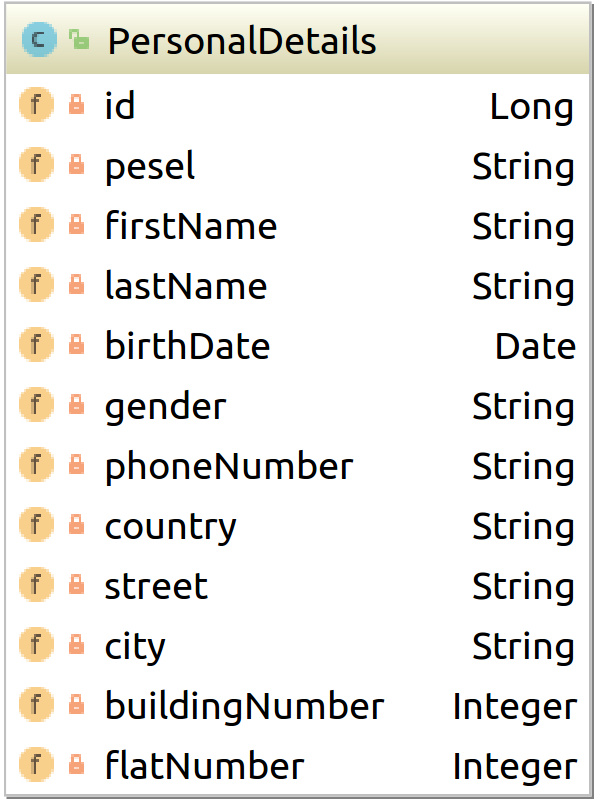
\includegraphics[width=0.7\textwidth]{PersonalDetails}
        \caption{Ta encja dotyczy zarówno lekarza i pacjenta}
    \end{figure}
    \paragraph{User} - dane użytkownika 
    \begin{figure}[H]
    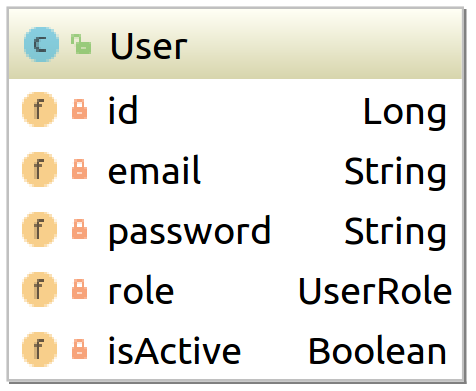
\includegraphics[width=0.7\textwidth]{User}
    \caption{powiązane z \emph{Account}}
    \end{figure}
    \paragraph{Specialization} - specjalizacja lekarza 
    \begin{figure}[H]
    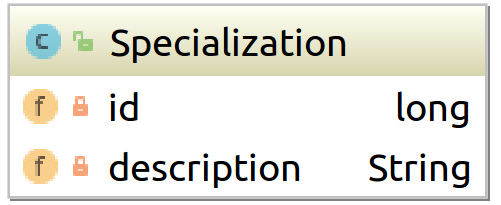
\includegraphics[width=0.7\textwidth]{Specialization}
    \end{figure}
\subsubsection{Powiązanie modelowanych encji}
\paragraph{Wersja zwinięta} - Schemat bez widocznych pól
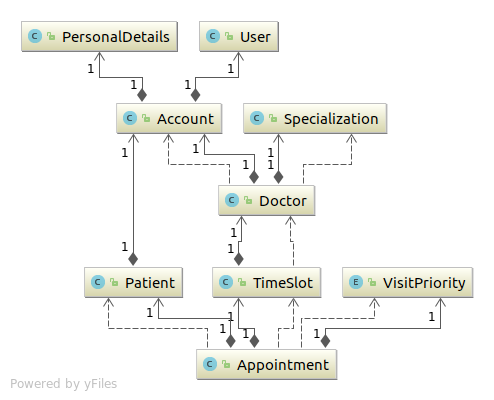
\includegraphics[width=\textwidth]{java-entities-small}
\paragraph{Wersja rozwinięta} - Schemat z widocznymi polami \\
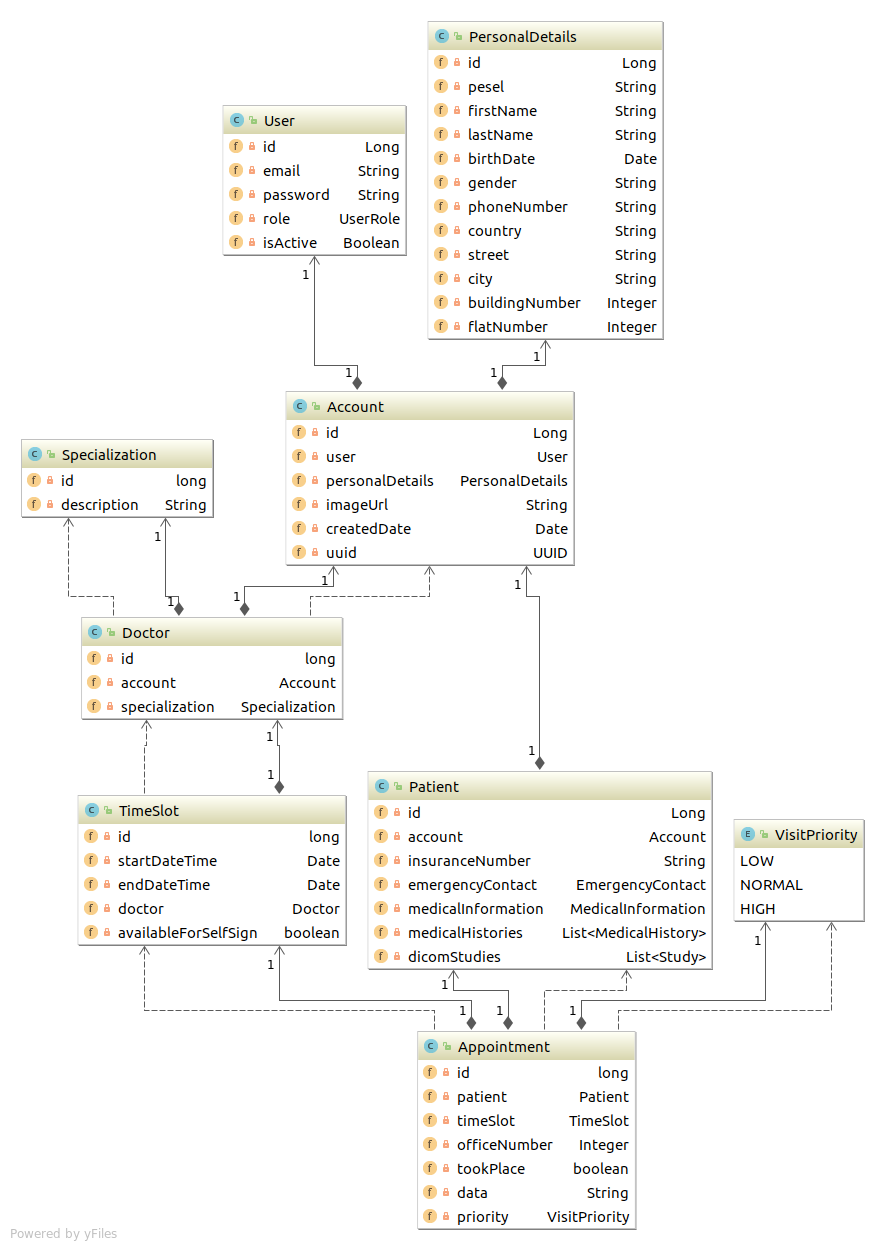
\includegraphics[width=\textwidth]{java-entities-big}

\subsubsection{Obsługa zapytań}
\paragraph{Schemat} -  
obsługa zapytań HTTP przychodzących do serwera ma w większości przypadków następujący przebieg (opisany we wstępie):
\begin{enumerate}
  \item \emph{Kontroler} odbiera zapytanie HTTP i przekazuje serwisowi
  \item \emph{Serwis} sprawdza poprawność zapytania i wykonuje pod-zapytania do repozytorium
  \item \emph{Repozytorium} pobiera potrzebne dane z bazy danych i zwraca serwisowi
  \item \emph{Serwis} przekształca dane otrzymane od repozytorium w odpowiedź na zapytanie i przekazuje odpowiedź kontrolerowi
  \item \emph{Kontroler} odsyła odpowiedź po HTTP
\end{enumerate}

\paragraph{Przykład - getTimeSlotById} - zapytanie o dane \emph{TimeSlot}-u na podstawie jego \emph{ID}
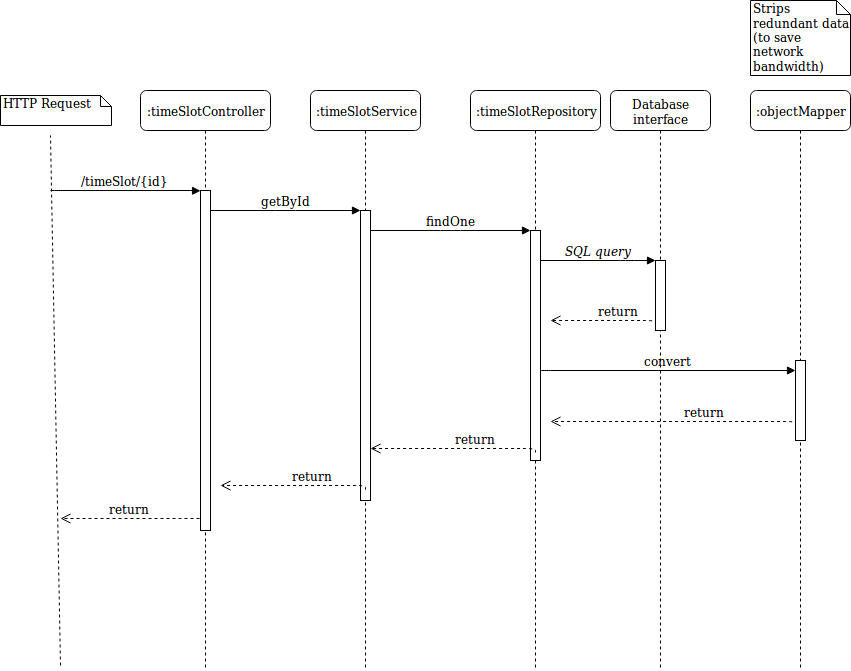
\includegraphics[width=\textwidth]{timeSlotById}

\paragraph{Przykład - getInIntervalForDoctor} - zapytanie o listę \emph{TimeSlot}-ów dla danego doktora w zadanym przedziale czasownym. \\
Schemat opisany powyżej jest na tyle ogólny że równie dobrze modeluje prostrze zapytanie \emph{getTimeSlotById} jak i bardziej skomplikowane \emph{getInIntervalForDoctor}. Różnica w implementacji występuje na poziomie \emph{repozytorium}, które musi wykonać odpowiednio inne zapytania do bazy danych i \emph{serwisu} który inaczej sprawdza poprawność danych
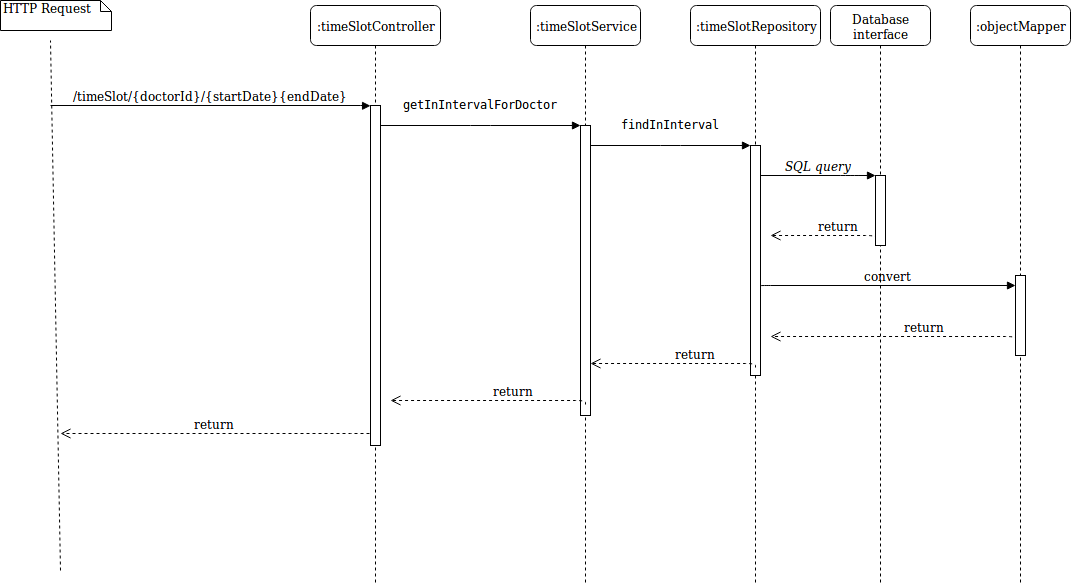
\includegraphics[width=\textwidth]{inIntervalDorDoctor}

\subsection{Aplikacja front-endowa}
\subsubsection{Technologie}
\paragraph{Angular 2} - zręby aplikacji przeglądarkowej. Umożliwiają:
\begin{itemize}
    \item wysyłanie i odbieranie zapytań HTTP
    \item dynamiczną zmianę zawartości strony internetowej
\end{itemize}
\subsubsection{Serwisy}
Serwisy służą do wysyłania zapytań HTTP. Ich metody zwracają \emph{Promise}. Serwisy służące rejestracji pacjentów:
\begin{itemize}
    \item authentication service
    \item appointment service
    \item doctor service
    \item google calendar service
    \item patient service
    \item timeSlot service
    \item user service
\end{itemize}
\paragraph{Zależności między serwisami}{
 Graf pokazuje których serwisów trzeba użyć any uzyskać całość danych na temat danej encji. \\
 Na przykład aby uzyskać całość danych na temat \emph{Appointment} trzeba znać \emph{TimeSlot}, \emph{Doctor}-a przyjmującego wizytę i \emph{Patient}-a zapisanego na wizytę.
 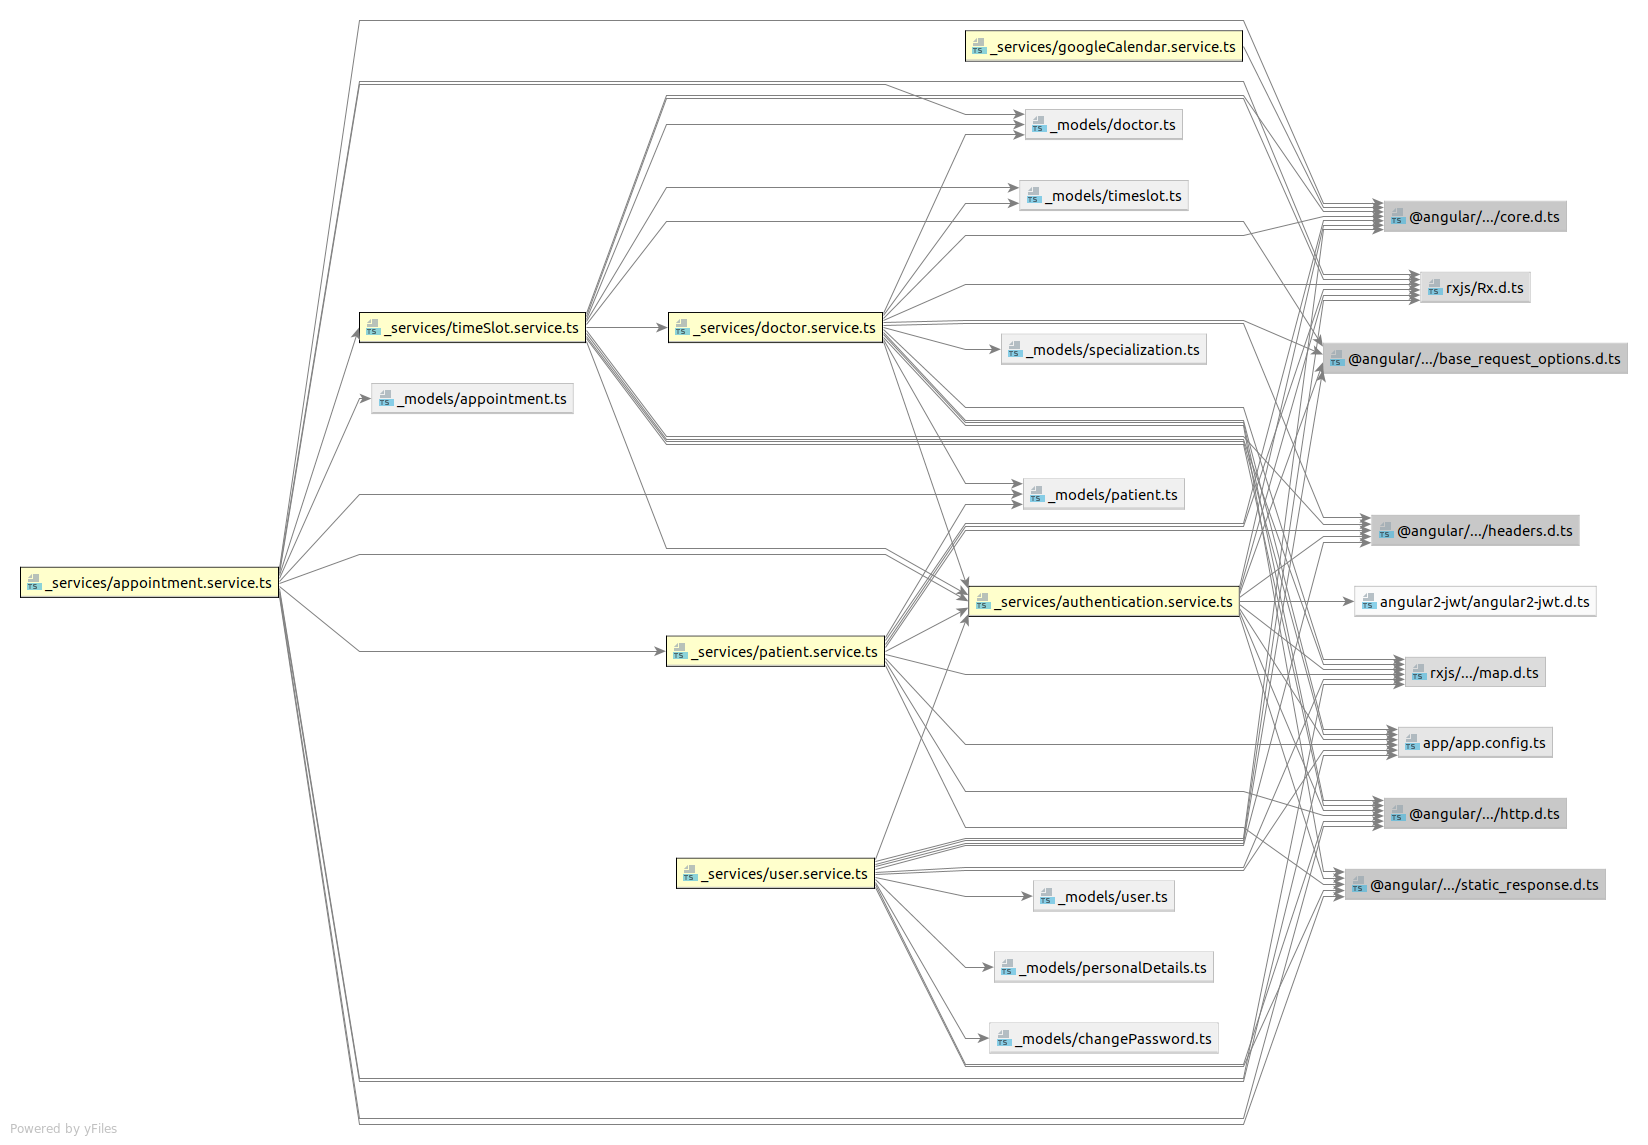
\includegraphics[width=\textwidth]{services-dep}
}

\subsubsection{Kalendarz terminów}
Kalendarz jest centralną częścią frontowej części systemu rejestracji
\paragraph{Diagram zależności} pokazuje wszystkie zależności komponentu kalendarza
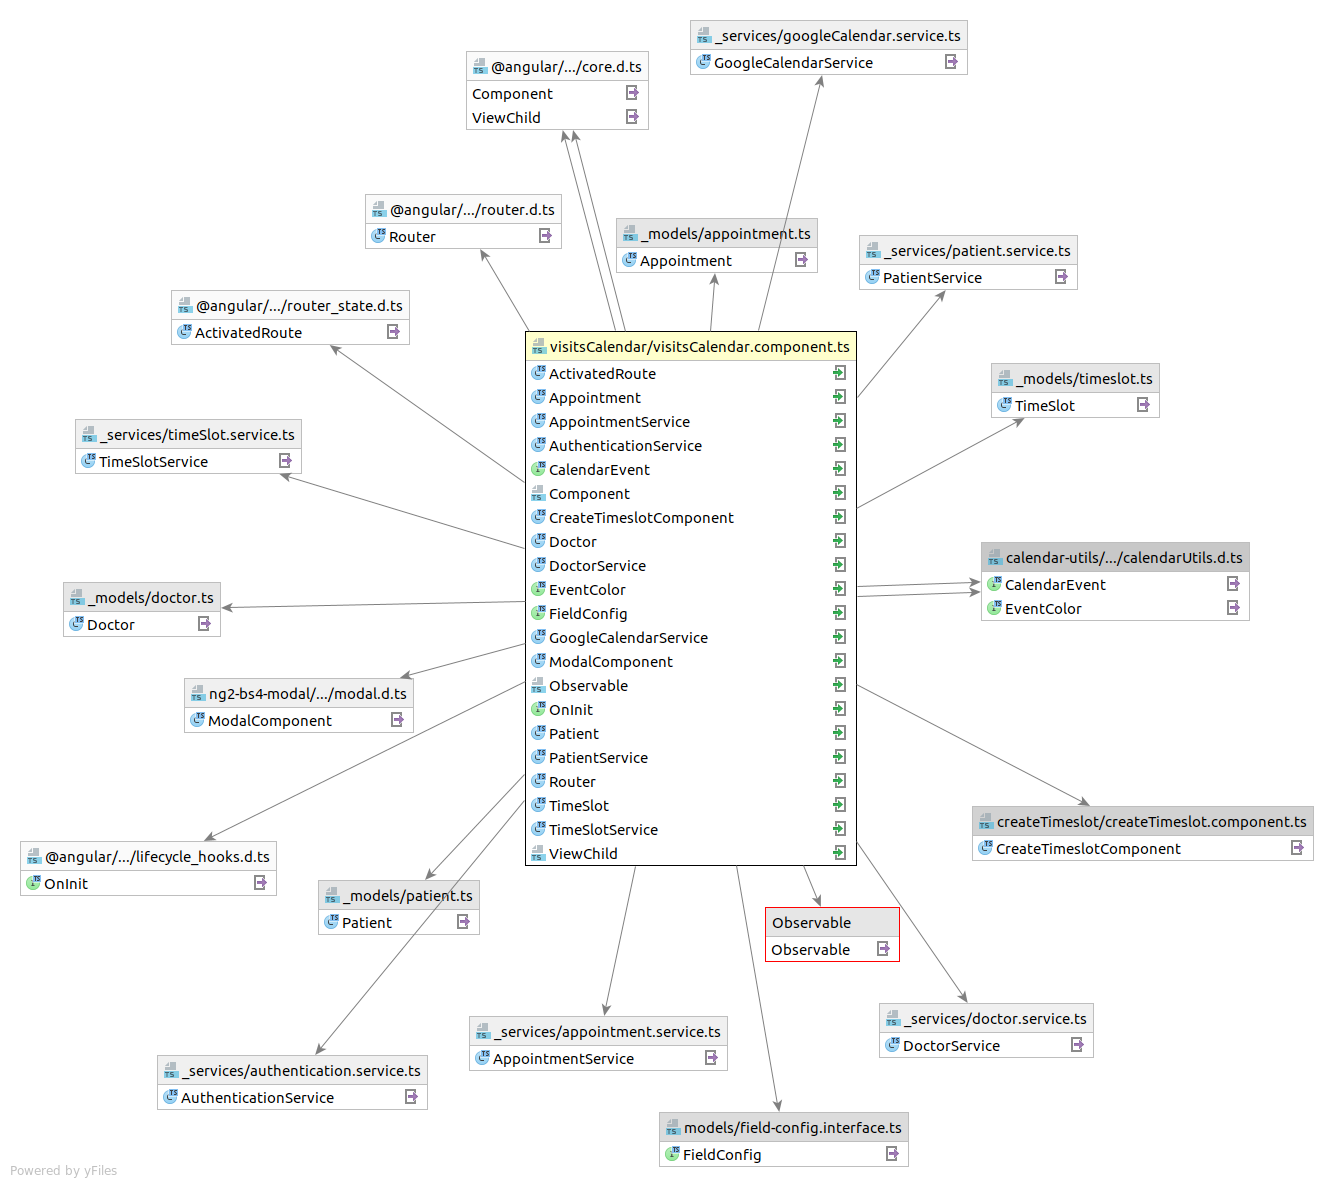
\includegraphics[width=\textwidth]{visitsCalendar_dep}
\paragraph{Inicjalizacja kalendarza}
Inicjalizacja wygląda inaczej w zależności od tego kto otwiera widok kalendarza.
\begin{itemize}
    \item Pacjent \\
     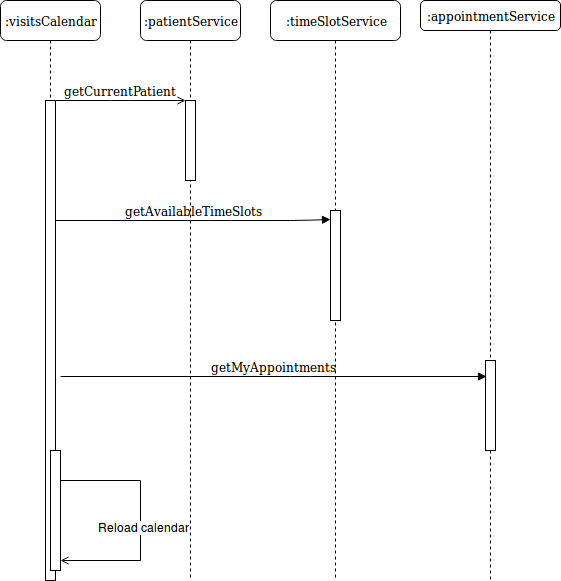
\includegraphics[width=\textwidth]{patient-init-cal}
    \item Doktor \\
    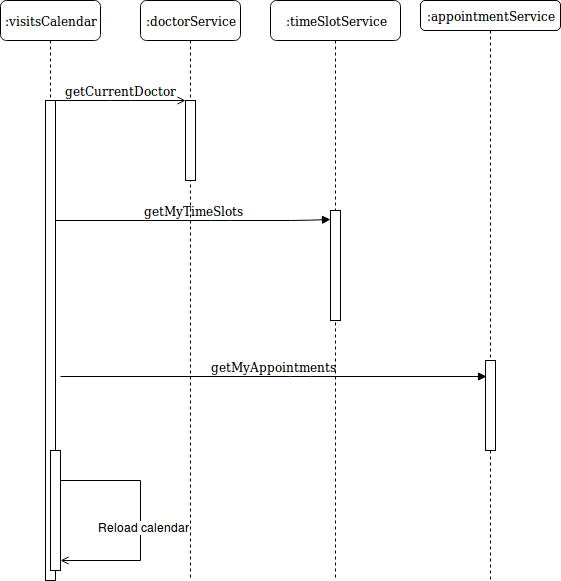
\includegraphics[width=\textwidth]{doctor-init-cal}
    \item Recepcjonistka \\
    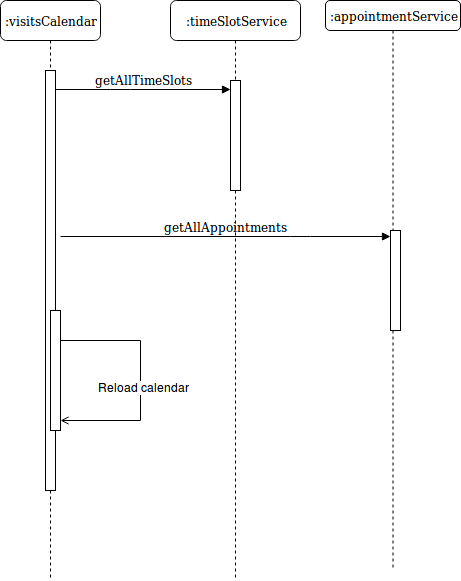
\includegraphics[width=\textwidth]{cal-recep-init}
\end{itemize}

%\paragraph{Zapis i modyfikacja danych}


\paragraph{Eksport terminów z kalendarza do 'Google Calendar'\footnote{Specyfikacja API znajduje się \href{https://www.googleapis.com/discovery/v1/apis/calendar/v3/rest}{tutaj}}} odbywa się wg schematu
\begin{enumerate}
    \item Zaloguj się - użytkownik zostaje przekierowany na stronę logowania Google, po zalogowaniu aplikacja otrzymuje jego token oAuth
    \item Dodaj wydarzenie do kalendarza
    \item Wyloguj się - token jest unieważniany
\end{enumerate}


\subsubsection{Formularze}
Formularze do tworzenia pacjentów, doktorów, terminów wizyt itp. są oparte o komponent \emph{DynamicForm} autorstwa powiązanego zespołu \emph{Health Manager}.
Ich konfiguracją jest lista JSON-owa. Przykład dla tworzenia dostępnych terminów (\emph{createTimeslot.component.ts})
\begin{verbatim}
    [
        {
            type: 'select',
            label: 'Doctor',
            name: 'doctor',
            placeholder: 'Select a doctor',
            options: []
        },
        {
            type: 'date',
            label: 'Start Date-time',
            name: 'startDateTime'
        },
        {
            type: 'date',
            label: 'End Date-time',
            name: 'endDateTime'
        },
        {
            type: 'checkbox',
            label: 'Available for self-sign',
            name: 'availableForSelfSign',
            value: true
        },
        {
            label: 'Submit',
            name: 'submit',
            type: 'button'
        }
    ];
\end{verbatim}
Każdy obiekt na liście konfigurującej odpowiada jednemu komponentowi do wprowadzania danych. Obiekty listy konfiguracji muszą mieć pola:
\begin{itemize}
    \item type - typ komponentu, może przyjmować wartości: 'select', 'date', 'checkbox', 'input', 'button'.
    \item label - nazwa widocza dla użytkownika, dowolny ciąg znaków
    \item name - nazwa która będzie identyfikowała komponent w kodzie, niewidoczna dla użytkownika
    \item value [opcjonalne] - domyślna wartość dla komponentu. Dostępne wartości zależą od rodzaju komponentu
\end{itemize}

\subsection{Komunikacja aplikacji przeglądarkowej i serwerowej}
Aplikacja przeglądarkowa i serwerowa komunikują się przez protokół HTTP (sposób nazywany czasem \emph{RESTowym API}. W treści zapytań jest JSON.
\paragraph{Przykład komunikacji:}{
\begin{enumerate}
  \item Lekarz, korzystając z aplikacji klienckiej, wysyła zapytanie o umówiony termin wizyty wysyłając HTTP GET na adres server-addr:8080/appointments/123. "123" to numer identyfikacyjny umówionej wizyty.
  \item Serwer zwraca odpowiedź
\begin{verbatim}
{    
  id: 123,
  patientId: 32,
  timeSlotId: 432,
  tookPlace: false,
  officeNumber: 10,
  data: "Podejrzenie shizofrenii bezobjawowej!",
  priority: LOW
}
\end{verbatim}
\end{enumerate}


Wykaz formatu zapytań i odpowiedzi znajduje się w załączniku
}

\section{Organizacja pracy}
%\section{Work organization}
\label{sec:organizacja-pracy}

\emph{Struktura zespołu (role poszczególnych osób), krótki opis i
  uzasadnienie przyjętej metodyki i/lub kolejności prac, planowane i
  zrealizowane etapy prac ze wskazaniem udziału poszczególnych
  członków zespołu, wykorzystane praktyki i narzędzia w zarządzaniu
  projektem.}
  
\subsection{Strunktura zespołu}
\subsubsection{Hierarchia zarządzania}
W zepole wyróżniony jest przywódca. Wyróżnianie innych funkcji wydało nam się zbędne.
\begin{itemize}
    \item Wojciech Karpiel - szef, odpowiedzialny za komunikację z Klientem i współpracującymi zespołami
    \item Fiip Galas - członek zespołu
    \item Michał Hamuda - członek zespołu
\end{itemize}
\subsubsection{Podział technologiczny}
Rozważaliśmy wprowadzenie podziału ze względu na kompetencje techniczne, czyli:
\begin{itemize}
    \item Osoba zajmująca się stroną serwerową
    \item Osoba zajmująca się aplikacją przeglądarkową
\end{itemize}
Uznaliśmy to za zabyteczne ponieważ produkt składa się głównie z kodu front-endowego i taki podział funkcji spowodowałby nierównomierny podział prac. Zamiast tego każdy członek zespołu odpowiadał za stworzenie front-endowej i back-endowej części funkcjonalności którą wdrażał.

\subsection{Wyznaczanie i rozdział zadań}
Wykorzystywaliśmy Jira-ę, hostowaną przez IISG. Po każdym spotkaniu z Klientem szef zespołu przetwarzał wymagane przez Klienta funkcjonalności na Jira-owe bilety. Każde zadanie opisywało jedną funkcjonalność. Zadania były posortowane wegług ważności (to znaczy: funckjonalności które należało zaimplementować do następnego spotkania z klientem były najwyżej, najniżej były nasze pomysły których Klient nie wymagał). Członkowie zespołu, według czasu i możliwości, przypisywali sobie zadania i wykonywali je.
 \begin{figure}[H]
    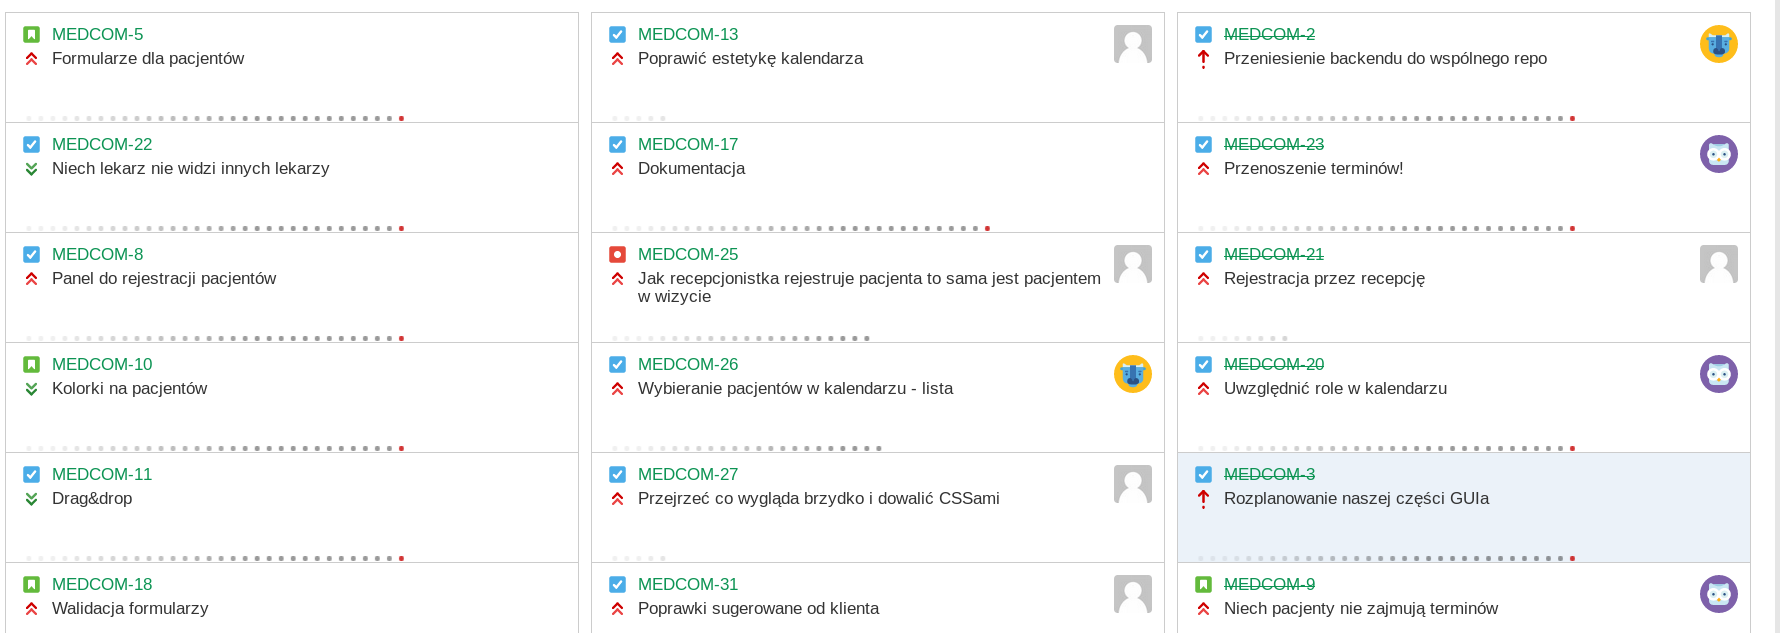
\includegraphics[width=0.7\textwidth]{jira-kanban}
    \caption{Tablica Kanbanowa projeku PRZEMEK - element zwinnej metodyki tworzenia oprogramowania}
    \end{figure}

\subsection{Sposób wykonywania zadań}
Produkt składa się de facto z dwóch powiązanych pod-projektów: części front-endowej i back-enbdowej. Te dwa pod-projekty były objęte systemem kontroli wersji Git. Dla każdego pod-projektu osobno członek zespołu tworzył Git-ową gałąź przypisaną funkcjonalności i na niej komitował kod wprowadzający funkcjowalność. Po zakończeniu pracy, pozostali członkowie zespołu przeglądali kod na gałęzi i ewentualnie prosili o wprowadzenie poprawek (code-review). Na końcu gałąź funkcjonalnościowa była dołączana do głównej gałęzi.

\subsection{Komunikacja z powiązanymi zespołami}
\subsubsection{Komunikacja bieżąca}
Do komunikacji bieżącej używaliśmy komunikatora Skype. Według potrzeb, umawialiśmy się na ta zwane call-e, podczas których przedstawiciele każdego z powiązanych zespołów omawiali stan prac i planowali przyszłą pracę.
\subsubsection{Wymiana wiedzy}
Używaliśmy Confluence-a, hostowanego przez IISG. Służył on jako pamięć długotrwała oraz punkt wymiany informacji między zespołami. Tam spisywaliśmy notatki ze spotkań (zarówno tych z Klientem jak i między-zespołowych), prowadziliśmy kalendarz przyszłych spotkań oraz spisywaliśmy różnorakie informacje które wydawały się nam przydatne. Do tego Confluence-a mieli dostęp również członkowie powiązanych zespołów.
 \begin{figure}[H]
    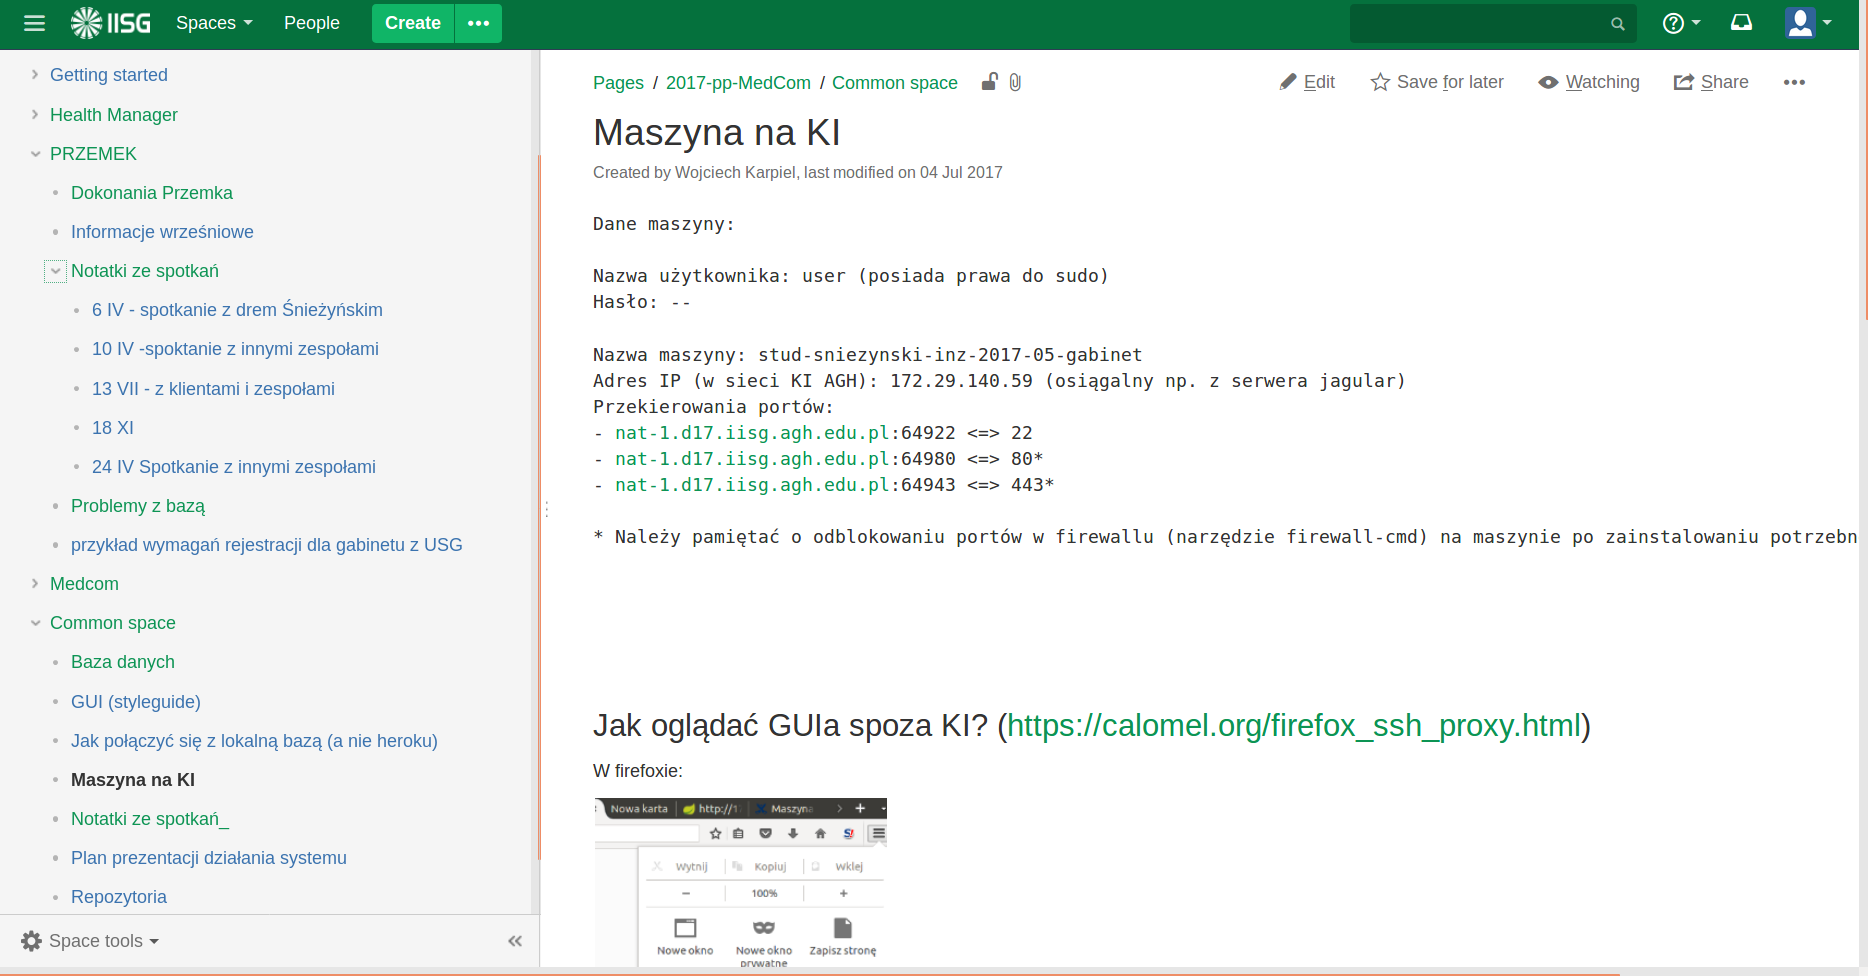
\includegraphics[width=0.7\textwidth]{confluence-maszyna}
    \caption{Strona na Confluence - oprogramowaniu wspomagającym współpracę przy tworzeniu oprogramowania}
    \end{figure}
    
\subsection{Spotkania z Klientem}
Naszym Klientem był dr Bartłomiej Śnieżyński, natomiast Klientem powiązanych zespołów był dr Piotr Nawrocki. Razem z zespołami powiązanymi prosiliśmy naszych Klientów o wspólne spotkania (3 zespoły i 2 Klientów), na co nasi Klienci chętnie przystali. Taka organizacja spotkań ułatwiła koordynację i integrację zespołów.
  
  
\subsection{Podział prac ze względu na osobę wykonującą}
\begin{center}
  \begin{tabular}{ | l | l | }
    \hline
    %%% TODO
    %%% WSZYSTKO TRZEBA POROZDZIELAĆ NA JAK NAJDROBNIEJSZE SZCZEGÓLIKI
    %%% TAK ŻEBY WYSZŁO ŻE DUŻO ZROBILIŚMY xDD
    %%% TA CZĘŚĆ JEST WAŻNA BO O NIĄ NAWROCKI PROSIŁ 2 RAZY
    %%% można np dopisać kto jakie endpointy dodawał
    Wynik pracy & Osoba wykonująca \\ \hline \hline
    Prototyp  porzucany front-endu\footnote{Nie został w żadnej części wykorzystany we właściwym produkcie ze względu na niezgodność wykorzystanych technologii} & Mihał Hamuda \\ \hline
    Prototyp back-endu\footnote{Został częściowo wykorzystany we właściwym produkcie} & Filip Galas  \\ \hline
    Wizja projektu\footnote{Tworzona na potrzeby Pracowni projektowej} & Wojciech Karpiel \\ \hline
    Kalendarz wizyt & Michał Hamuda \\ \hline
    Możliwość przenoszenia terminów & Wojciech Karpiel \\ \hline
    Integracja kalendarza z \emph{Google Calendar} & Filip Galas \\ \hline
    Rejestracja pacjenta przez recepcjonistkę & Michał Hamuda \\ \hline
    Uwzględnienie roli użytkownika (\emph{aktora}) w kalendarzu & Wojciech Karpiel \\ \hline
    Możliwość dodawania terminów wizyt & Filip Galas \\ \hline
    Ładny wygląd i estetyka aplikacji & Michał Hamuda \\ \hline
    Możliwość oznaczenia terminu jako dostępnego do rejestracji tylko przez recepcję & Wojciech Karpiel \\ \hline
    Możliwość zapisywania się na wizytę & Wojciech Karpiel \\ \hline
    Oznaczanie zajętych i wolnych wizyt kolorem w kalendarzu & Wojciech Karpiel \\ \hline
    Grafik pracy lekarzy & Wojciech Karpiel \\ \hline
    Usuwanie zaplanowanej wizyty & Wojciech Karpiel \\ \hline
    Usuwanie dostępnego terminu wizyty & Wojciech Karpiel \\ \hline
    Widok zarezerwowanych wizyt dla lekarza i pacjenta & Wojciech Karpiel \\ \hline
    Dodawanie wielu terminów lekarza na raz & Wojciech Karpiel \\ \hline
    Dokumentacja projektu & Wojciech Karpiel \\ \hline
    Poprawki do dokumentacji & Filip Galas \\ \hline
    Kontakty z Klientem & Wojciech Karpiel \\ \hline
    Synchronizacja między zespołami & Wojciech Karpiel \\ \hline
    Utrzymanie serwera (VM udzielona przez Klienta) z uruchomioną aplikacją & Wojciech Karpiel \\ \hline
  \end{tabular}
\end{center}
  %% Koniec organizacji pracy!



\section{Wyniki projektu}
%\section{Project results}

\label{sec:wyniki-projektu}

\emph{Wskazanie wyników projektu (co konkretnie udało się uzyskało:
  oprogramowanie, dokumentacja, raporty z testów/wdrożenia, itd.), prezentacja wyników
  i ocena ich użyteczności (jak zostało to zweryfikowane --- np.\ wnioski
  klienta/użytkownika, zrealizowane testy wydajnościowe, itd.),
  istniejce ograniczenia i propozycje dalszych prac.}

\subsection{Wymagania dla uruchomiania aplikacji}
\subsubsection{Wymagania techniczne dla klienta}
\begin{itemize}
  \item  Połączenie z serwerem Health-Menagera (zazwyczaj realizowane przez sieć Internet)
  \item Przeglądarka internetowa zdolna do obsługi ECMAScript-u w wersji 6 lub późniejszej (na przykład Mozilla Firefox w wersji 56.0)
\end{itemize}

\subsubsection{Wymagania techniczne dla serwera}
\begin{itemize}
    \item Połączenie z siecią komuterową w której znajdują się użytkownicy
    \item Java Runtime Environment w wersi 8 lub późniejszej (na przykład \href{https://www.java.com/pl/download/manual.jsp}{JRE firmy Oracle}
    \item Baza danych PostgreSQL
    \item Serwer HTTP Tomcat
\end{itemize}

\subsubsection{Wymagania techniczne dla programisty}
\begin{itemize}
    \item \href{https://www.npmjs.com/}{NPM - Next Popular Module}
    \item Java Developement Kit w wersi 8 lub późniejszej
    \item Gradle
    \item Baza danych Postgresql
\end{itemize}


\subsection{Konfiguracja aplikacji}
\subsubsection{Aplikacja przeglądarkowa}{Należy ustawić:
\begin{itemize}
    \item port na którym będzie wystawione GUI (przez HTTP)
    \item Adres end-pointu back-endowego
\end{itemize}}
\subsubsection{Aplikacja serwerowa}{Należy ustawić:
\begin{itemize}
    \item Parametry połączenia z bazą danych
\end{itemize}}
\paragraph{Baza danych}{Prawidłowo skonfigurowana aplikacja serwerowa powinna utworzyć schemat bazy danych w przypadku jego nieistnienia}


\subsection{Przewodnik użytkownika}
%%TODO: Nie ma ogarniętego wdrożenia aplikacji więc nie ma co opowiadać administratorowi
%\subsubsection{Administrator}
%    \paragraph{Rejestracja użytkownika}{}
%    \paragraph{Utrzymanie aplikacji}{}
\subsubsection{Pacjent}
%    \paragraph{Rejestracja}{}
    \paragraph{Logowanie}{
    Pacjent otrzymuje od rejestrującej recepcjonistki dane dostępowe do swojego konta. \\
    \begin{enumerate}
        \item Za pomocą przeglądarki internetowej połącz się z serwerem udostępniającym usługę
        \item Wpisz adres e-mail podany przy rejestracji oraz swoje hasło
    \end{enumerate}
    \begin{figure}[H]
        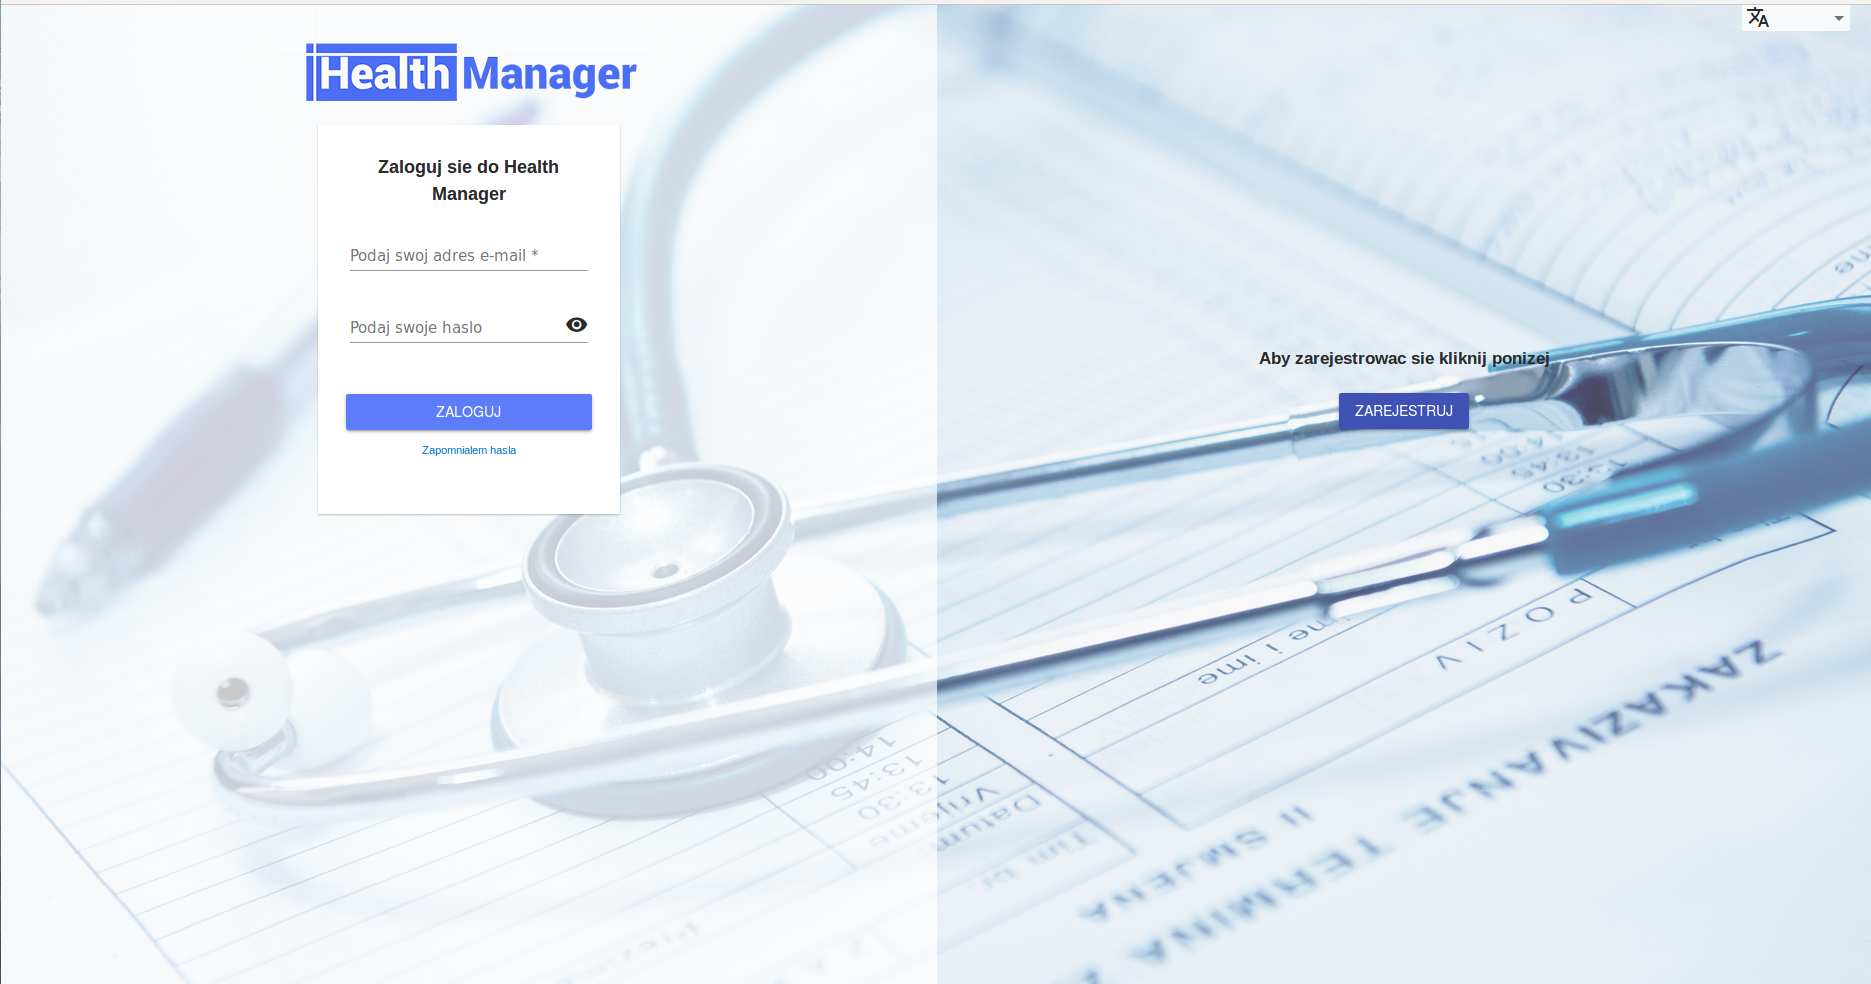
\includegraphics[width=0.7\textwidth]{gui-loginpage}
        \caption{Strona logowania}
    \end{figure}
    Po zalogowaniu użytkownik zostaje przeniesiony na pulpit
    \begin{figure}[H]
        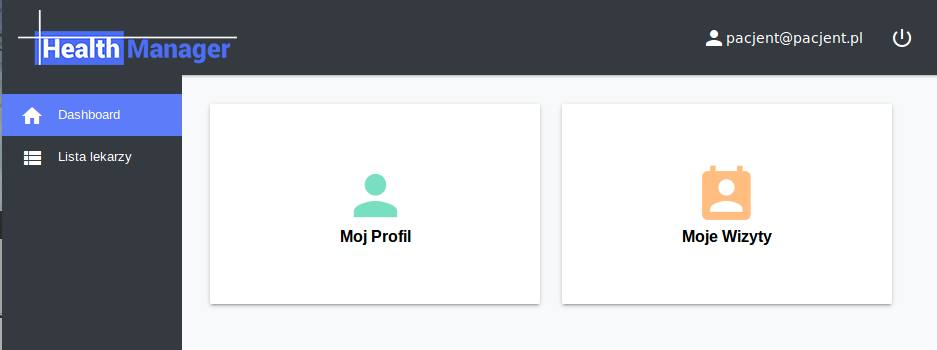
\includegraphics[width=0.7\textwidth]{gui-patient-dashboard}
        \caption{Pulpit pacjenta}
    \end{figure}
        
    }
    \paragraph{Moje wizyty}{Lista umówionych wizyt, pozwala wyświetlić wizyty przyszłe i już odbyte w zależności od wybranego przedziału czasowego. Dostarczane informacje:
    \begin{itemize}
        \item Termin wizyty
        \item Imię i nazwisko lekarza
        \item Numer gabinetu
        \item odnośnik do szczegółowych informacji na temat wizyty
    \end{itemize}
    %%TODO WSTAWIĆ NOWY OBRAZEK JAK BĘDZIE NAPRAWIONY BUG ŻE PACJENT NIE MOŻE OTRZYMAĆ INFO O SAMYM SOBIE
        \begin{figure}[H]
        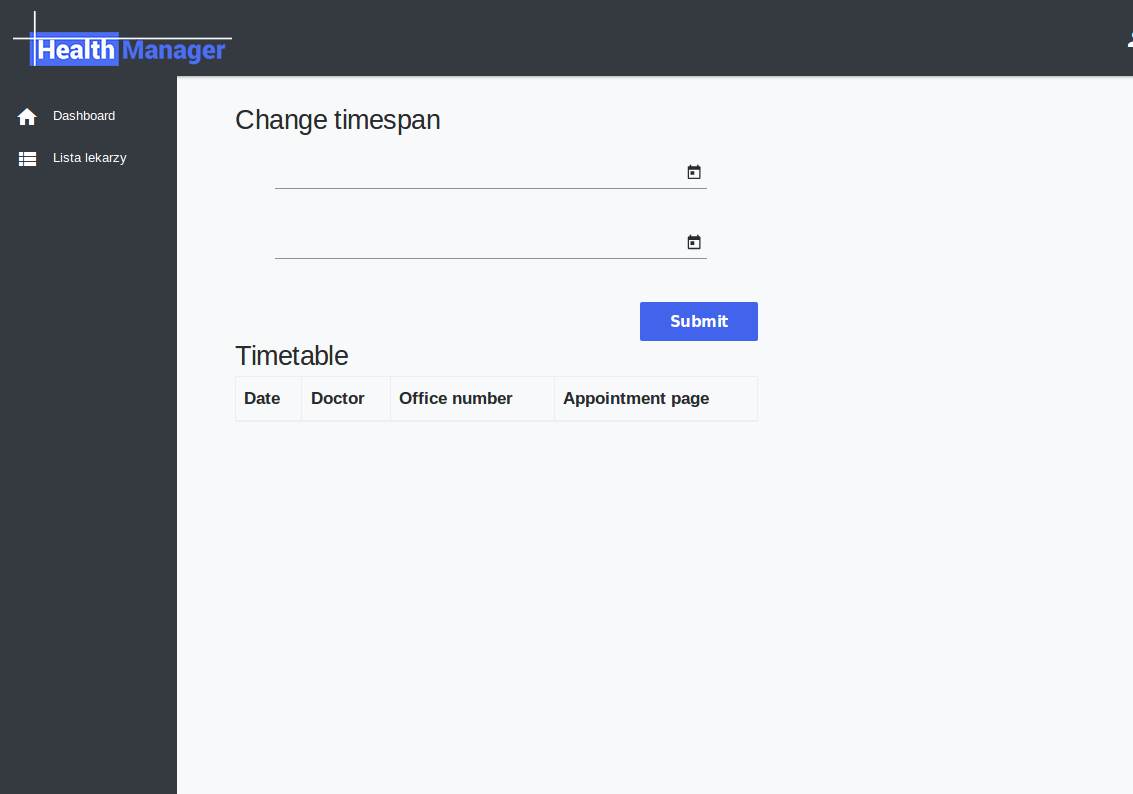
\includegraphics[width=0.7\textwidth]{gui-patient-my-visits}
        \caption{Lista umówionych wizyt pacjenta}
    \end{figure}    
    }
    \paragraph{Lista lekarzy} pozwala na umówienie się na wizytę z konkretnym lekarzem
    \begin{figure}[H]
        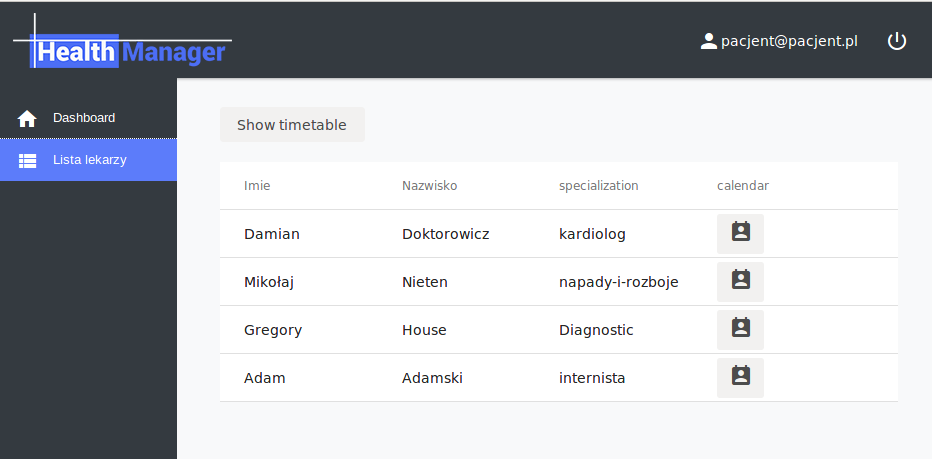
\includegraphics[width=0.7\textwidth]{gui-doctor-list}
        \caption{Lista lekarzy}
    \end{figure}
    Aby zobaczyć dostępne terminy dla danego lekarza należy kliknąć ikonkę kalendarzyka w wierszu zawierającym nazwisko danego lekarza
    \paragraph{Kalendarz lekarza}{ pozwala zobaczyć
    \begin{itemize}
        \item Dostępne terminy wizyt - oznaczone kolorem niebieskim
        \item Umówione wizyty - oznaczone kolorem czerwonym
    \end{itemize}
    
    
    \begin{figure}[H]
        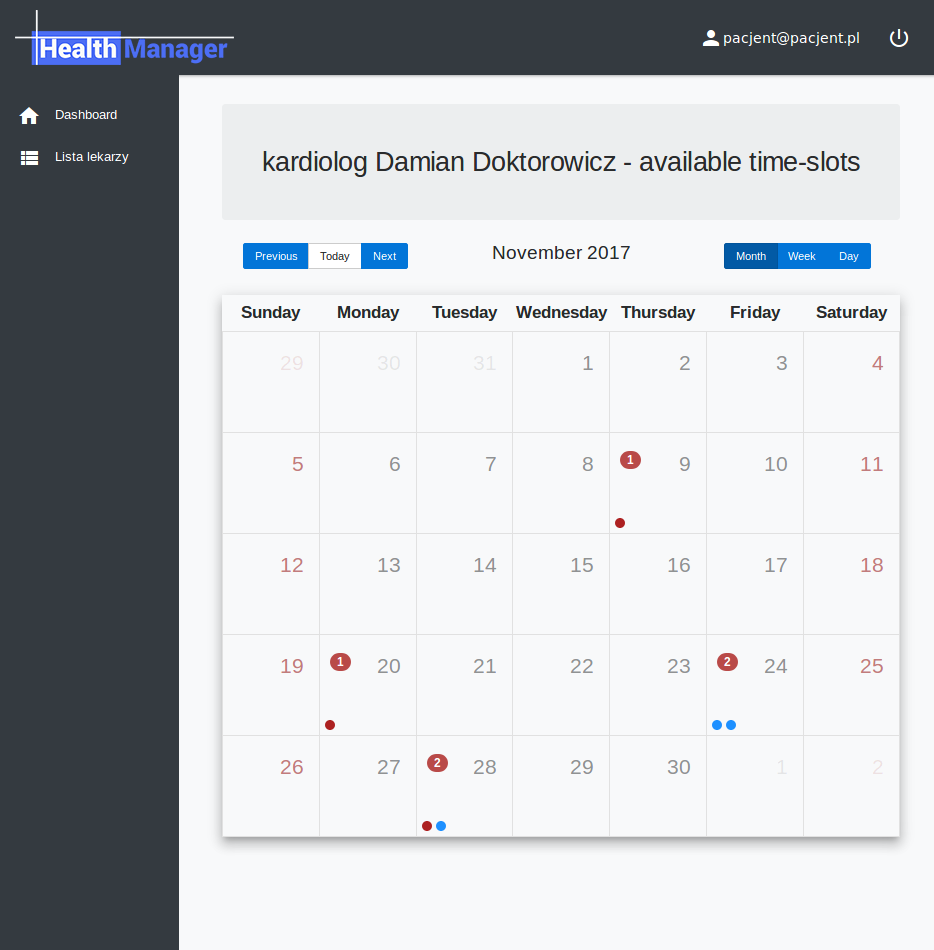
\includegraphics[width=0.7\textwidth]{gui-calendar-patient-month}
        \caption{Kalendarz lekarza - widok miesiąca}
    \end{figure}    
    \begin{figure}[H]
        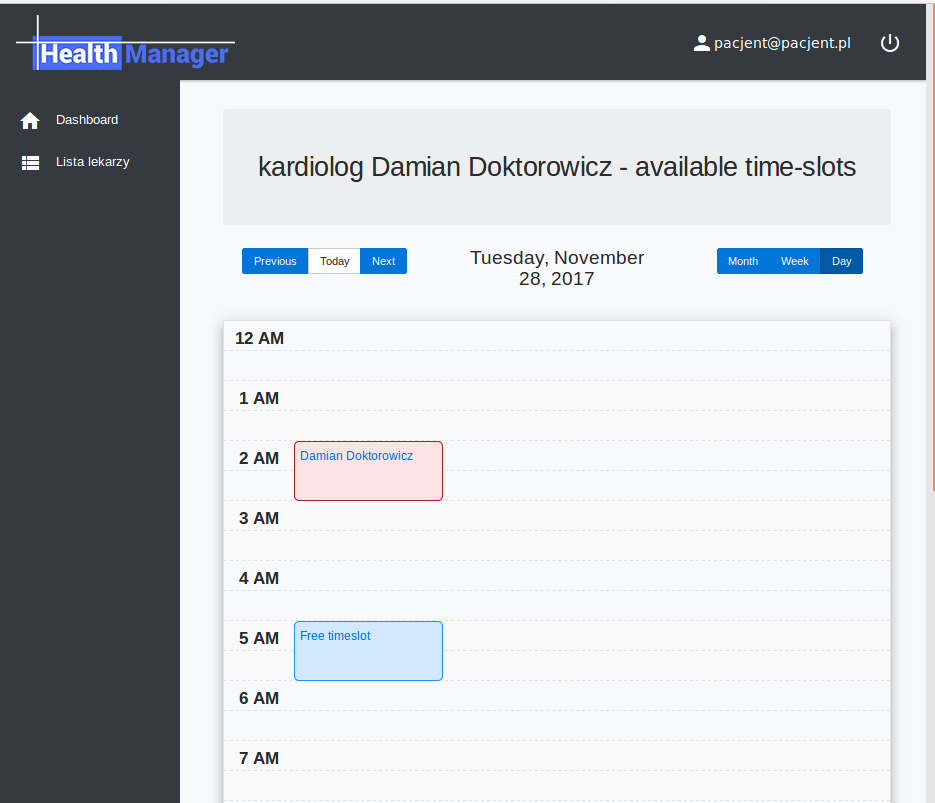
\includegraphics[width=0.7\textwidth]{gui-calendar-patient-day}
        \caption{Kalendarz lekarza - widok dnia}
    \end{figure}    
    }
    \paragraph{Zapis na wizytę}{  - Po kliknięciu na dostępny (oznaczony kolorem niebieskim) termin w widoku kalendarza można się na umówić na wizytę klikając zielony przycisk \emph{Zapisz}. Powód wizyty (bądź inną informację do przekazania lekarzowi) można wpisać w pole \emph{Powód wizyty}
    \begin{figure}[H]
        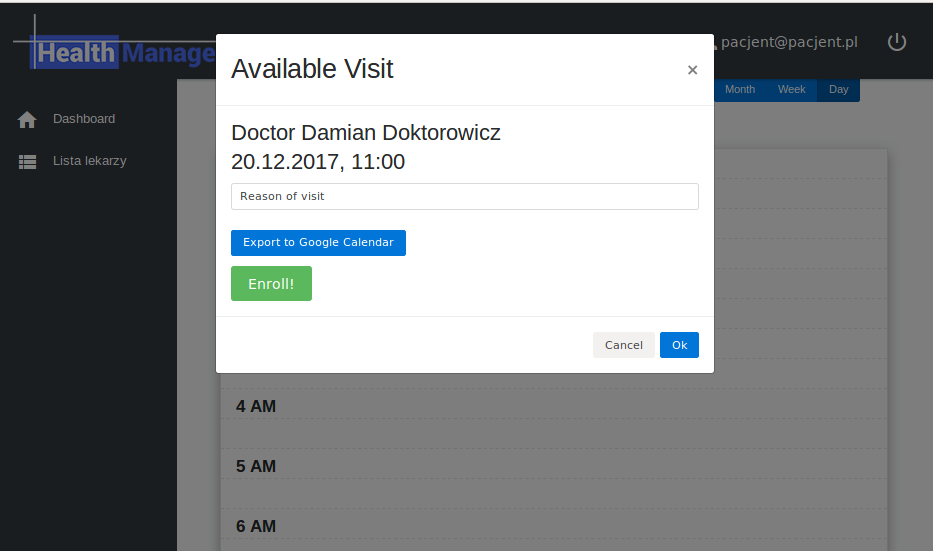
\includegraphics[width=0.7\textwidth]{gui-patient-unenrolled-visit-window}
        \caption{Okno zapisu na wizytę}
    \end{figure}    
    }
    \paragraph{Odwołanie wizyty}{- Po kliknięciu na planowany (oznaczony kolorem czerwonym) termin w widoku kalendarza można odwołać wizytę klikając \emph{Odwołaj}        
        \begin{figure}[H]
        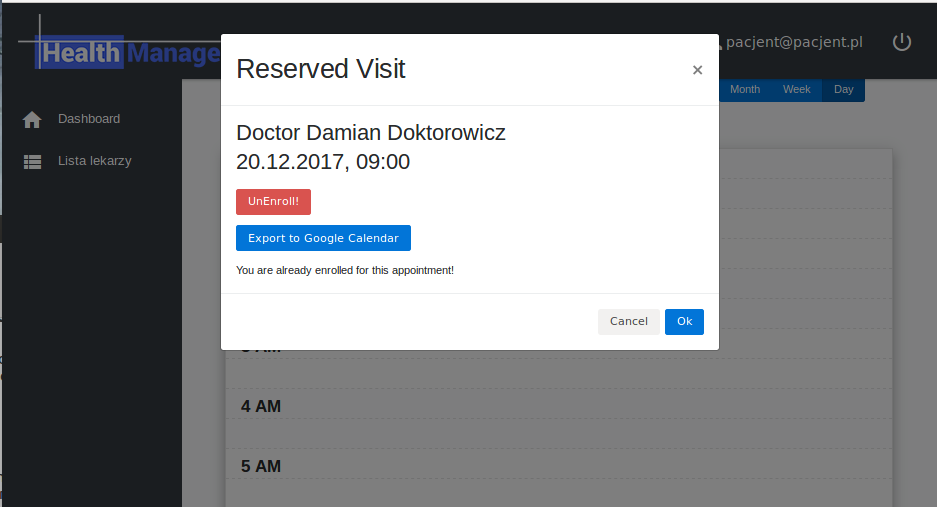
\includegraphics[width=0.7\textwidth]{gui-patient-enrolled-visit-window}
        \caption{Okno zapisanej wizyty}
        \end{figure}  
    }
    \paragraph{Eksport do kalendarza Google.}{ W oknie zapisanej wizyty i oknie zapisu można wyeksportować termin do kalendarza Google klikając \emph{Eksportuj do kalendarza Google}.
    \begin{enumerate}
      \item Kliknij \emph{Eksportuj do kalendarza Google}
      \item W otorzonym okienku uzupełnij swoje dane logowania do konta Google
    \end{enumerate}
       \begin{figure}[H]
        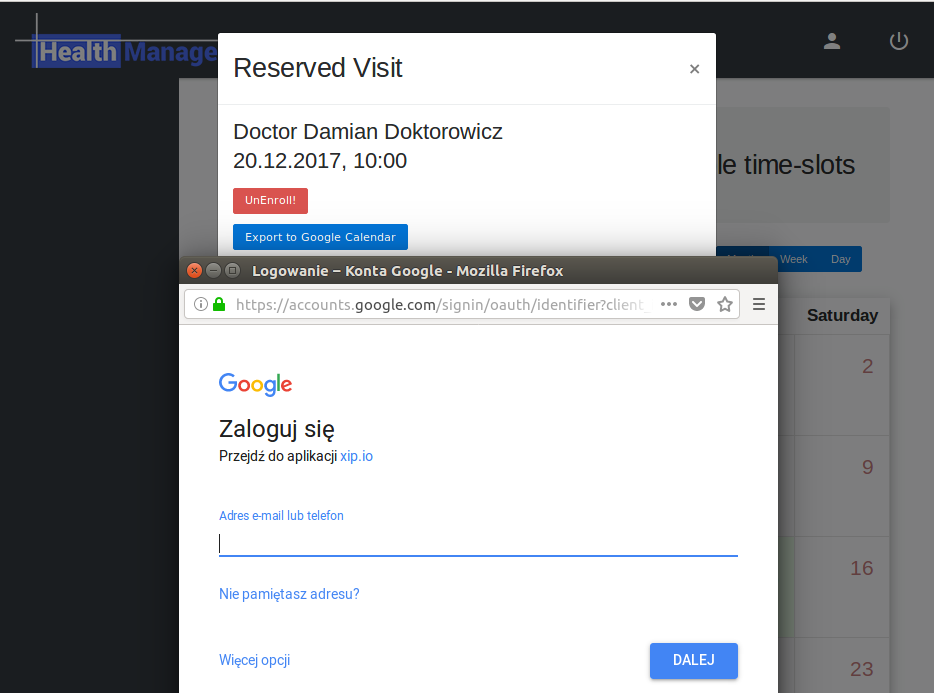
\includegraphics[width=0.7\textwidth]{gui-google-export}
        \caption{Eksport do kalendarza Google}
        \end{figure}  
    }
\subsubsection{Lekarz}
    \paragraph{Ustalanie grafiku}{}
    \paragraph{Drukowanie grafiku}{}
    \paragraph{Ustalanie terminów}{}
    \paragraph{Rejestracja pacjenta}{}
    \paragraph{Eksport kalendarza}{}
\subsubsection{Recepcjonistka}
    \paragraph{Rejestracja pacjenta}{}
    \paragraph{Zmiana terminu wizyty}{}


\listoffigures 
\listoftables
%%%%% KONIEC %%%%%%
% o ile to mozliwe prosze uzywac odwolan \cite w konkretnych miejscach a nie \nocite

\nocite{artykul2011,ksiazka2011,narzedzie2011,projekt2011}

\bibliography{bibliografia}

\end{document}
